%! TEX program = xelatex

\chapter{Quantum Gate Learning}
\label{Section:GateLearning}

Synthesising target quantum operations is pivotal is a number of contexts in quantum information science, for example in quantum simulation~\cite{feynman1982simulating,lloyd1996universal}, quantum computation~\cite{feynman1982simulating,deutsch1985quantum,gottesman1998theory,nielsen2002quantum,ladd2010quantum}.
In particular, unitary gates play a key role in the majority of schemes for quantum computation and quantum algorithms, and more generally are a fundamental component of most quantum information protocols.

Implementing a given target unitary gate can however often be a daunting task. Different techiniques can be used to achieve this, depending on the particular experimental context and constraints.
For example, in a photonics context, one often has access to a toolbox of elementary components, such as beamsplitters and phaseshifters, which are used to build up more complex operations.
In this context, to built a complex operation $U$, one is tasked with finding a suitable combination of such elementary (generally unitary) operations $G_i$ such that $U=\prod_i G_i$. Given a fixed set of \textit{elementary gates} $\{G_i\}_i$, finding a suitable combination of these gates that results in the target operation $U$ is highly nontrivial, and is a task often referred to as the \textit{gate compilation} or \textit{gate synthesis} problem~\cite{mottonen2004quantum,nielsen2006quantum,loke2014optqc,loke2016optqc,nakajima2009synthesis,maslov2017basic,swaddle2017generating}. \highlight{(add more citations)}
\highlight{are there other experimental contexts in which it is common to have such \textit{black boxes} that are composed together?}
Solving gate compilation problems is especially important in the light of the recent significant experimental advances in the construction of experimental quantum devices, especially superconducting~\cite{devoret2013superconducting} and ion trap~\cite{blatt2008entangled,debnath2016demonstration} architectures.

A completely different type of problem is the one faced when, instead of a discrete set of gates, one is able to tune continuous parameters of an underlying dynamics.
In other words, it can be the case that the experimenter has access to some parameters $\bs\lambda$ of the system \textit{Hamiltonian} $H_{\bs\lambda}$, and wants to find the values of $\bs\lambda$ to achieve some target dynamics.
One might for example be interested in driving a fixed input to a fixed target output, or in obtaining a full effective evolution via tuning the dynamics.
In this kind of scenario, it is also common to allow for \textit{time-dependent} dynamics. This makes it much easier, in general, to achieve different types of evolutions, but at the same times makes the resulting optimisation problem that much harder, as one then has to look for an optimal \textit{function} $t\mapsto\bs\lambda(t)$, rather than just an optimal value $\bs\lambda\in\mathbb R^n$.
This types of problems are usually referred to as \textit{quantum (optimal) control} problems.
\highlight{quantum control refs}



\begin{itemize}
    \item \textbf{\textit{You can also mix these types of problems together, and/or add ancillary resources.}}
    \item The third situation is ours: we want to tune the dynamics to getter better black boxes.
    \item What's the advantages of doing it our way?
\end{itemize}

We are \cite{innocenti2018supervised}.

Open problems and solutions, literature.

\section{Standard techniques for gate engineering, previous work}
\highlight{I'm not actually sure we want this section}

\section{Time-independent dynamics for target gates}

Here, we explore a different approach to devise target unitary evolutions. More specifically, we ask the following question: is there a way to implement a given target gate \textit{without} decomposing it as a sequence of simpler gates, \textit{and} without using a time-dependent dynamics, \textit{and} without the aid of additional ancillary resources?
In other words, given a target operation $\calU$, and a set of possible candidate Hamiltonians $\calH[\bullet]\equiv \{\calH_{\bs\lambda}\}_{\bs\lambda}\subseteq\on{Herm}$\footnote{Here, $\on{Herm}\equiv\on{Herm}(N)$ is the set of Hermitian $N\times N$ matrices with complex entries, for some integer $N\ge2$. The dimension $N$ will be taken to be understood from the context.},
can we find a \textit{time-independent} Hamiltonian $\calH\in\calH[\bullet]$ such that, at some time $t$, we have $\calU = e^{-it \calH}$?
\footnote{Throughout this work, we will only consider the cases of operations and Hamiltonians acting on \textit{finite-dimensional} systems (generally sets of qubits).}
Note that if no restriction is imposed on $\calH[\bullet]$, then the problem is always trivially solvable. Indeed, writing $\calU$ in its eigendecomposition as
$\calU=\sum_k e^{i\varphi_k}\PP_k$ for some set of orthogonal projectors $\PP_j\PP_k=\delta_{jk}\PP_j$ with $\sum_k\PP_k=I_N$ and phases $\varphi_k\in\RR$, then any $\calH$ of the form
$\calH = -\sum_k \varphi_k\mathbb P_k$ satisfies $e^{-i\calH}=\cal U$.
\highlight{Do we want to prove this linear algebra stuff at some point?}
The interesting cases, both from a theoretical and practical perspective, are therefore when $\calH[\bullet]$ is constrained to have some specific structure.
Here, we will consider the case of $\calH[\bullet]$ being a set of Hamiltonians parametrised by a number of continuous parameters (in other words, it's taken to be a parametrised surface in $\on{Herm}(N)$).
We will therefore always assume that there is a continuous mapping $\RR^\ell\ni\bs\lambda\mapsto\calH(\bs\lambda)\in\on{Herm}$ such that $\calH[\bullet]=\calH(I)$ for some $I\subseteq\RR^\ell$ (which will be usually taken to equal $\RR^\ell$ for simplicity).

We can also consider the time $t$ as part of the definition of $\calH$, which amounts to a rescaling of the energy levels. We can therefore also assume $t=1$ in the following. Finally, to ease the calculations, we will consider the equivalent problem of finding $\calH$ such that $\calU=e^{i\cal H}$ (with the plus sign), as the solutions to one can be seamlessly translated into solutions to the other problem.

For concreteness, let us analyse what happens when we try to find Hamiltonian generators for a few common two- and three-qubit gates, namely the CNOT and the Toffoli gate.
\highlight{Ensure no other gates are added in the examples}
\begin{example}[label=ex:eigendecomposition_cnot]
Assume that the target operation is $\CNOT$: the two-qubit unitary gate which flips the second qubit conditionally to the value of the first one.
In matrix notation, this reads
\begin{equation}
    \on{CNOT} \equiv\begin{pmatrix}1&0&0&0 \\ 0&1&0&0 \\ 0&0&0&1\\0&0&1&0\end{pmatrix} =
    \PP_0\otimes I_2 + \PP_1\otimes X,
\end{equation}
where $\PP_k\equiv\ketbra k$ and $X$ is the Pauli $X$ gate.
The eigendecomposition of this matrix is
\begin{equation}
    \on{CNOT} =
    \ketbra{0,0} + \ketbra{0,1} + \ketbra{1,+} - \ketbra{1,-}.
    \label{eq:cnot_eigendecomposition}
\end{equation}
A more expressive way to write~\cref{eq:cnot_eigendecomposition} is by introducing the projectors $X^\pm\equiv(1\pm X)/2$, and the similarly defined $Y^\pm$ and $Z^\pm$ (here, $X,Y,Z$ denote the one-qubit Pauli matrices).
\Cref{eq:cnot_eigendecomposition} is then equivalently written as
\begin{equation}
    \on{CNOT} =
    Z^+_1 Z^+_2 + Z^+_1 Z^-_2
    + Z^-_1 X^+_2
    - Z^-_1 X^-_2
    = Z_1^+ + Z_1^- X_2^+ - Z_1^- X_2^-.
    \label{eq:cnot_eigdecomp_with_paulis}
\end{equation}
The eigenvalues are therefore $\lambda_{1,2,3}=1$ and $\lambda_4=-1$.
Can this gate be obtained via a two-qubit time-independent Hamiltonian $\calH$?
Consider for the purpose a general parametrisation of the possible two-qubit Hamiltonians, which we can write using the set of Pauli matrices on the two qubits as operatorial basis:
\begin{equation}
    \calH({\bs\lambda}) =
    \sum_{j,k=0}^4 \lambda_{j,k} \sigma^j_1\sigma^k_2.
\end{equation}
Given the decomposition of~\cref{eq:cnot_eigdecomp_with_paulis}, it is natural to use as an Ansatz for $\calH(\bs\lambda)$ an expression bearing the same eigenstructure as the CNOT. Let us therefore write
\begin{equation}
    \calH(\bs\lambda) = \lambda_1 Z_1^+ + \lambda_2 Z_1^- X_2^+ + \lambda_3 Z_1^- X_2^-.
\end{equation}
Finding $\bs\lambda\equiv(\lambda_1,\lambda_2,\lambda_3)$ such that $e^{i\calH}=\CNOT$ is then quite easy: just use $\lambda_1=\lambda_2=0$ and $\lambda_3=2\pi$. Indeed, as it is easy to check, $e^{\pi i Z_1^- X_2^-} = \CNOT$.
The natural next question is then: is this the \textbf{only} such $\calH$? It is straightforward to see that the answer is negative: for example, it is also true that $e^{\pi i n Z_1^- X_2^-}=\CNOT$ for any $n\in\ZZ$.
It is less trivial to get a complete characterisation of the solution set.
Indeed, as will be shown in~\cref{sec:solutions_matrix_equation_f(A)=B}, there is a rich set of solutions for these types of matrix equations.
\end{example}

\begin{example}[label={ex:eigendecomposition_Toffoli}]
Consider now the \textbf{Toffoli gate}, which is a three-qubit gate which flips the third qubit conditionally to the first two qubits being in the $\ket1$ state.\highlight{Ensure Toffoli was defined before, or add relevant references here.}
More explicitly, this means
\begin{equation}
    \Toff =
    \PP_0\otimes I_4 + \PP_1\otimes\CNOT
    \equiv
    \begin{pmatrix}
        I_4 & \mathbb{0}_4 \\
        \mathbb 0_4 & \CNOT
    \end{pmatrix}.
    % \begin{pmatrix}
    %     1&0&0&0&0&0&0&0 \\
    %     0&1&0&0&0&0&0&0 \\
    %     0&0&1&0&0&0&0&0 \\
    %     0&0&0&1&0&0&0&0 \\
    %     0&0&0&0&1&0&0&0 \\
    %     0&0&0&0&0&1&0&0 \\
    %     0&0&0&0&0&0&0&1 \\
    %     0&0&0&0&0&0&1&0
    % \end{pmatrix}
\end{equation}
In terms of projectors onto eigenvalues of (products of) Pauli matrices, we have
\begin{equation}
    \Toff = Z_1^+ + Z_1^- Z_2^+ + Z_1^- Z_2^- X_3^+ - Z_1^- Z_2^- X_3^-.
\end{equation}
The eigenvalues of $\Toff$ are thus readily seen to be $+1$ with multiplicity $7$, and $-1$ with multiplicity $1$.
A possible $\calH$ such that $e^{i\cal H}=\Toff$ is then $\calH=\pi Z_1^- Z_2^- X_3^-$.
Note how expanding this Hamiltonian we get
\begin{equation}
    \calH = \frac{\pi}{8}\left[
        I - (Z_1 - Z_2 - X_3)
        + (Z_1 Z_2 + Z_1 X_3 + Z_2 X_3)
        - Z_1 Z_2 X_3
    \right],
\end{equation}
which contains three-qubit interaction terms (the $Z_1 Z_2 X_3$ factor). While this is to be expected , as the Toffoli is a non-trivial three-qubit gate, these kinds of terms make practically implementing these Hamiltonians significantly harder.
Indeed, natural interactions, and in particular interactions that can be easily implemented in experiments, generally \highlight{can we promote this to \textbf{always}?} involve only one- and two-qubit interaction terms.
It is then natural to wonder about whether this is a \textbf{necessary} feature of time-independent generators of the Toffoli gates.
As will be shown in the following sections, the answer is in fact that yes, it is possible to find time-independent Hamiltonians that generate a Toffoli gate \textbf{and} only use up to two-qubit interactions.
\end{example}

As shown in~\cref{ex:eigendecomposition_cnot,ex:eigendecomposition_Toffoli}, looking for Hermitian generators of few-qubit gates is not a fairly straightforward task. There are, however, two notable issues with the type of analysis conducted so far:
\begin{enumerate}
    \item It lacks in generality: while finding specific generators essentially amounts to computing the eigendecomposition of the target $\calU$, and then the logarithm of the eigenvalues, this says nothing about whether such procedure provides the most general kind of Hamiltonian generator for the given gate. In other words, can \textit{all} generators $\calH$ be obtained this way?
    \item We have no control over the kind of generators that we obtain with this procedure. For example, in~\cref{ex:eigendecomposition_cnot} we obtained generators containing two-qubit interactions of the form $Z_1 X_2$. Does this mean that this type of interaction term is \textit{necessary} to generate a CNOT? Or is there instead some Hamiltonian that can still generate the CNOT without using such terms?
    Similar questions arise in~\cref{ex:eigendecomposition_Toffoli}.
\end{enumerate}
To address these issues, we will study the underlying mathematical problem in more depth. As it turns out, we can divide such analysis in two parts. In~\cref{sec:solutions_matrix_equation_f(A)=B}, we show how to find general solutions to inverse matrix equations of the form $f(A)=B$. Then, in~\cref{sec:constraints_on_interaction_pars}, we present a way to bring additional constraints on the interaction terms into the discussion.
\highlight{to review this part probably}

\section{Solutions of the matrix equation \texorpdfstring{$f(A)=B$}{f(A)=B}}
\label{sec:solutions_matrix_equation_f(A)=B}
Let $A,B$ be normal matrices such that $f(A)=B$ for some function $f$ (assumed to be regular on the spectrum of $A$), with $f(A)$ defined as usual on the eigenvalues of $A$.
In this section we will provide a full characterisation of the set of solutions $A\in f^{-1}(B)$ .

Explicitly, $f(A)=B$ amounts to
\begin{equation}
    \sum_j \lambda_j^B \PP_j^B = \sum_k f(\lambda_k^A) \PP_k^A,
    \label{eq:f(A)=B_eigendecomp_proof}
\end{equation}
where $\PP_k^{A} (\PP_k^{B})$ are the projectors onto the corresponding eigenspaces of $A$ and $B$, so that
$A\PP_k^A=\lambda_k \PP_k^A$, and similarly for $B$.
Because both sides of~\cref{eq:f(A)=B_eigendecomp_proof} define the eigendecomposition of some (normal) operator, by the uniqueness of the eigendecompositions it follows that $\lambda_j^B=f(\lambda_j^A)$ and $\PP_j^B=\PP_j^A$.
What is interesting about this is that it means that the relation $f(A)=B$ puts strong constraints on the eigenstructure of $A$: the eigenspaces of $A$ must be the same as those of $B$.

Consider now the problem of finding a matrix $A$ such that $f(A)=B$, for some predetermined mapping $f$.
If $f$ is injective (at least on $f^{-1}(\sigma(B))$), then, by our above argument, it follows that $A$ is uniquely determined. Indeed, we the condition would then be
\begin{equation}
    \sum_j \lambda_j^B \PP_j = \sum_j f(\lambda_j^A) \PP_j,
\end{equation}
which can only be true for $\lambda_j^A = f^{-1}(\lambda_j^B)$.
However, because we are considering here matrices and functions defined over $\CC$, most interesting cases will correspond to \textit{non-injective} functions $f$\footnote{Indeed, the only entire, injective functions $\CC\to\CC$ are the linear mappings $z\mapsto az+b$ for some $a,b\in\CC$.}. The case $f(z)=e^z$, which is the one with which we will be mostly concerned with for the gate learning problem, is one such case of non-injective function.

When $f$ is non-injective, there can be multiple $A$ such that $f(A)=B$. There are two main reasons for this, one fairly evidence, and the other one less so.
Clearly, being $f$ not injective, for any given eigenvalue $\lambda_j^B$ there can be multiple $\lambda$ such that $f(\lambda)=\lambda_j^B$. This is indeed the only source of non-uniqueness whenever the eigenspaces of $B$ are all one-dimensional (equivalently, the projetors $\PP_k^B$ in~\cref{eq:f(A)=B_eigendecomp_proof} have all unit trace).
However, whenever there are eigenspaces of dimension greater than one, there are multiple (infinite) ways to write a corresponding projector $\PP$ as sum of unit-trace projectors. Assume for example that $\Tr\PP=d$, and let $\PP_k$ be a set of $d$ unit-trace projectors such that $\PP=\sum_{k=1}^d \PP_k$. Let $U$ be an arbitrary operator that is unitary in the range of $\PP$.
Then we have
\begin{equation}
    \PP=U^\dagger \PP U =\sum_{k=1}^d U^\dagger \PP_k U
    \equiv \sum_{k=1}^d \tildePP_k,
    \label{eq:rewriting_proj_with_rotated_projs}
\end{equation}
where we defined the ``rotated projectors'' $\tildePP_k\equiv U^\dagger \PP U$.
While this rewriting is ininfluent in~\cref{eq:rewriting_proj_with_rotated_projs}, such rotations of the degenerate eigenspaces turn out to be of great relevance when looking for solutions of $f(A)=B$.
To see this, let us consider again~\cref{eq:f(A)=B_eigendecomp_proof}, and focus on a single eigenspace $\PP_j^B$ such that $\Tr\PP_j^B=d_j>1$ (assuming $B$ has one), and write an arbitrary decomposition of $\PP_j^B$ in terms of on unit-trace projectors as $\PP_j^B=\sum_{\ell=1}^{d_j}\PP^B_{j,\ell}$.
Let $\{\lambda_{j,\ell}\}_{\ell=1}^{d_j}\subseteq f^{-1}(\lambda_j^B)$ be a subset of inverses of $\lambda_j^B$. Then, any $A$ which has $\lambda_{j,\ell}$ as eigenvalues within the eigenspace $\PP_j^B$ is a suitable solution for $f^{-1}(B)$.
In other words, we have
\begin{equation}
    A \equiv \sum_j \sum_{\ell=1}^{d_j} \lambda_{j,\ell} \PP_{j,\ell}\in f^{-1}(B),
    \quad \forall \lambda_{j,\ell}\in\CC \text{ with } f(\lambda_{j,\ell})=\lambda_j^B.
    \label{eq:general_form_f-1B}
\end{equation}
Note how this means that $f^{-1}(B)$ \textit{can break the degeneracies in $B$} thanks for the non-injectivity of $f$.

Let us give now a few concrete examples of the freedom allowed by the degeneracies.

\begin{example}[label={ex:solutions_f(A)=I2}]
Consider the two-dimensional identity matrix $I_2$, and an arbitrary complex function $f$ defined on the complex unit. \textbf{What is then the set of matrices $A$ such that $f(A)=I_2$?}
Note that $I_2=P+Q$ for any pair of orthogonal projectors $P,Q$, and $\lambda P + \mu Q\in f^{-1}(I_2)$ for any $\lambda,\mu\in f^{-1}(1)$.
This can be equivalently stated saying that, for any pair of orthonormal states $\ket u$ and $\ket v$, we have
$\lambda \ketbra u + \mu \ketbra v\in f^{-1}(I_2)$.
Going further, we parametrise the set of all such vectors writing (we can define the vectors up to an overall phase, as we are only interested in the corresponding projectors):
\begin{equation}
    \begin{cases}
    \ket u =\cos\alpha\ket 0+e^{i\theta}\sin\alpha \ket 1, \\
    \ket v =-e^{-i\theta}\sin\alpha\ket 0 + \cos\alpha\ket 1.
\end{cases}
\end{equation}
This provides us with a parametrisation for the set of solutions $f^{-1}(B)$:
\begin{equation}
\begin{aligned}
    A = &\lambda\left(\cos^2(\alpha) \PP_0 + \sin^2(\alpha) \PP_1 + \sin(2\alpha)\Re[e^{i\theta}\ketbra{1}{0}]\right) \\
    +&\mu\left(
        \sin^2(\alpha) \PP_0 + \cos^2(\alpha) \PP_1 - \sin(2\alpha)\Re[e^{i\theta}\ketbra{1}{0}]
    \right),
\end{aligned}
\end{equation}
or in matrix form,
\begin{equation}
    A = \begin{pmatrix}
        \lambda \cos^2(\alpha)+\mu\sin^2(\alpha) &
        \frac12 e^{-i\theta} \sin(2\alpha) (\lambda-\mu) \\ 
        \frac12 e^{i\theta} \sin(2\alpha) (\lambda-\mu) &
        \lambda \sin^2(\alpha)+\mu\cos^2(\alpha)
    \end{pmatrix}.
    \label{eq:explicit_inverse_f(A)_matrix_form}
\end{equation}
We conclude that any such $A$ is such that $f(A)=I_2$, as long as $f(\lambda)=f(\mu)=1$, and that this form covers the set of all possible normal matrices satisfying this equation.
Whenever $\lambda=\mu$,~\cref{eq:explicit_inverse_f(A)_matrix_form} reduces to $A=\lambda I_2$, which is the trivial solution. When $\lambda\neq\mu$, however, it is less obvious that the corresponding matrix in~\cref{eq:explicit_inverse_f(A)_matrix_form} satisfies $f(A)=I_2$.
\end{example}

\begin{example}[label={ex:solutions_f(A)=I_3}]
\highlight{To decide where to put this crap.}

Consider how to split the eigenspace of the three-dimensional identity $I_3$.
This essentially amounts to the problem of parametrising a set of three orthonormal complex vectors. For the purpose, let us write them as
\begin{equation}
\begin{cases}
    \ket{u_1} = \cos(\alpha)\ket0
    + e^{i\theta}\sin(\alpha)\cos(\beta)\ket1
    + e^{i\varphi}\sin(\alpha)\sin(\beta)\ket2, \\
    \ket{u_2} = \cos(\alpha)\ket0
    + e^{i\theta}\sin(\alpha)\cos(\beta)\ket1
    + e^{i\varphi}\sin(\alpha)\sin(\beta)\ket2, \\
\end{cases}
\end{equation}
\highlight{Actually, there might not be a general nice way to parametrise such sets of vectors!}
\end{example}

\begin{example}[label={ex:solutions_e^A=I2}]
Picking up from~\cref{ex:solutions_f(A)=I2}, let us analyse the solutions to $f(A)=I_2$ when $f(z)=e^z$.
Then $f^{-1}(1)=2\pi i\ZZ$, and the set of solutions becomes
\begin{equation}
    A_{\alpha,\theta;n,m} = 2\pi i
    \begin{pmatrix}
        n \cos^2(\alpha)+m\sin^2(\alpha) &
        \frac12 e^{-i\theta} \sin(2\alpha) (n-m) \\ 
        \frac12 e^{i\theta} \sin(2\alpha) (n-m) &
        n \sin^2(\alpha)+m\cos^2(\alpha)
    \end{pmatrix},
\end{equation}
for all $n,m\in\ZZ$ and $\alpha,\theta\in\RR$.
\end{example}

\begin{example}[label={ex:cnot_generator_decomposition}]
We gave in~\cref{ex:eigendecomposition_cnot} a possible Hamiltonian generator for the CNOT gate.
Here, strong on the general characterisation of matrix inverses given in~\cref{eq:general_form_f-1B}, we work out a more general expression for the set of Hamiltonians $\calH$ such that $e^{i\calH}=\CNOT$.
Specialising~\cref{eq:general_form_f-1B} to the specific eigenstructure of $\CNOT$ (which we worked out in~\cref{ex:eigendecomposition_cnot}), we see that a generic (normal) generator for $\CNOT$ has the form
\begin{equation}
    \sum_{j=1}^3 \lambda_j \tildePP_j + \mu\PP_4,
\end{equation}
where
$\PP_4\equiv\ketbra 4\equiv\ketbra{1,-}$, the projectors 
$\{\tildePP_j\}_{j=1}^3$ define an arbitrary splitting of the degenerate eigenspace $\ker[(\CNOT-I_4)]$ into orthonormal vectors, and $\lambda_j,\mu\in\CC$ are such that $e^{i\lambda_j}=1$ and $e^{i\mu}=-1$.
These last conditions identify $\lambda_j\in2\pi\ZZ$ and $\mu\in\pi + 2\pi\ZZ$.
% \begin{equation}
%     \lambda_{j,\ell} = 2\pi n_{j,\ell},
%     \quad
%     \mu_\ell = \pi + 2\pi m_\ell,
%     \quad
%     n_{j,\ell},m_\ell\in\ZZ.
% \end{equation}
A generic generator for the CNOT can thus be written as
\begin{equation}
    \calH =
    2\pi\left[
    \sum_{j=1}^3 n_j \tildePP_j +
    \frac{1}{2} m\PP_4
    \right].
\end{equation}
It is worth stressing how the set of viable generators $\calH$ has both a discrete and a continuous degree of freedom.
\end{example}

In the rest of the thesis, we will focus on the case $f(A)\equiv e^{iA}$, which is case of relevance to find Hamiltonians generating target unitaries.

\section{Adding physical practical constraints}
\label{sec:constraints_on_interaction_pars}

In~\cref{sec:solutions_matrix_equation_f(A)=B} we described how to write the full set of solution for a matrix equation of the form $f(A)=B$.
In this section we will show how introducing further constraints on the type of interaction terms allowed in the final generator reveals a particularly daunting task.

To restrict the type of interaction terms allowed in the final generator, means to fix some set $\calP$ comprised of orthogonal Hermitian operators $\sigma_i$, and ask for a generator $\calH\in f^{-1}(\calU)$ such that $\calH$ is in the span of $\{\sigma_i\}_i$:
\begin{equation}
    \calH \in f^{-1}(\calU) \cap \on{Span}\calP.
\end{equation}
In the following, we will focus on the case  $f(A)\equiv e^{iA}$. \highlight{probably need to specify what is $f$ here}
A typical (but not necessary) choice for the $\sigma_i$ is the set of one- and two-qubit interaction terms $\calP_{\le2}$, defined as
\begin{equation}
    \calP_{\le2} \equiv \{ I, X_i,Y_i,Z_i, X_i Y_j, X_i Z_j, Y_i Z_j : \,\,i,j=1,2,3 \}.
\end{equation}
We thus have for example $X_i,Y_j\in\calP_{\le2}$ and $X_i Z_j\in\calP_{\le2}$, but $X_i Y_j Z_k\notin\calP_{\le2}$ for $i\neq j,i\neq k$ and $j\neq k$.

Given a candidate generator $\calH\in f^{-1}(\calU)$, one would therefore need to decompose $\calH$ in a basis containing the elements of $\calP$, and impose that all terms outside of this set are vanishing.
Given a target gate with eigendecomposition
$\calU=\sum_j e^{i\varphi_j}\PP_j$ with $\Tr\PP_j=d_j$ and $\sum_j d_j=2^n$ with $n$ the number of qubits, this would entail in practice finding bases for each $\on{Range}(\PP_j)$ built out of states $\{\ket*{u_{jk}}\}_{k=1}^{d_j}\subset \mathbb{CP}^{d_j}$, and integers $n_{jk}$, such that
\begin{equation}
    \sum_j\sum_{k=1}^{d_j} (\varphi_j + 2\pi n_{jk}) \PP[\ket*{u_{jk}}]
    \in \on{Span}_{\RR}\calP.
\end{equation}

\begin{example}[label={ex:cnot_physical_constraints}]
Let $\calU=\CNOT$, and consider a set of allowed interactions containing only single-qubit terms: $\calP_1\equiv\{X_i,Y_i,Z_i\}_{i\in\{1,2\}}$.
Is there an $\calH$ containing only interactions in $\calP_1$ and such that $e^{i\calH}=\CNOT$?

From a physical point of view, the answer should obviously be that no, there cannot be any such Hamiltonian, as that would mean that an entangling two-qubit gate can be obtained without having the qubits interact in any way.
Still, it is interesting to see if we can recover this result using the formalism introduced in the previous section, as a testbed to see it in action.
Consider then the decomposition given in~\cref{ex:cnot_generator_decomposition} for the CNOT:
\begin{equation}
    \calH =
    2\pi\left[
    \sum_{j=1}^3 n_j \tildePP_j +
    \frac{1}{2} m\PP_4
    \right],
\label{eq:cnotex_general_H_expr}
\end{equation}
where
$\PP_4\equiv Z_1^- X_2^-$ and $\tildePP_1,\tildePP_2,\tildePP_3$ define an arbitrary splitting of the eigenspace generated by $\ket{0,0},\ket{0,1}$ and $\ket{1,+}$.
Let us write down explicitly the decompositions of these projectors in terms of Pauli matrices:
\begin{equation}
\begin{cases}
    \tildePP_1 &= Z_1^+ Z_2^+ \,= \frac{1}{4} (I + Z_1 + Z_2 + Z_1 Z_2), \\
    \tildePP_2 &= Z_1^+ Z_2^- \,= \frac{1}{4} (I + Z_1 - Z_2 - Z_1 Z_2), \\
    \tildePP_3 &= Z_1^- X_2^+ = \frac{1}{4} (I - Z_1 + X_2 - Z_1 X_2), \\
    \PP_4 &= Z_1^- X_2^- = \frac{1}{4} (I - Z_1 - X_2 + Z_1 X_2),
\end{cases}
\end{equation}
where we made a canonical choice for the $\tildePP_i$.
Without exploiting the freedom given by the degeneracies, it is straightforward to see that it is not possible to find values for the $n_j\in\ZZ$ such annihilate the two qubit interaction terms, due to the $1/2$ factor in~\cref{eq:cnotex_general_H_expr}.
Indeed, expanding~\cref{eq:cnotex_general_H_expr} and focusing on the two-qubit interaction terms, we get
\begin{equation}
    \calH = (...) + \frac{2\pi}{4}\left[
    (n_1 - n_2) Z_1 Z_2 +
    (n_4/2 - n_3) Z_1 X_2
    \right].
\end{equation}
Remarkably, this shows how the $Z_1 X_2$ seems to be a necessary part of a generator, as there is no choice of $n_3,n_4\in\ZZ$ such that $n_4-2 n_3=0$.
Still, this does not rule out the possibility that for some other choice of $\tildePP_j$ it is possible.
The difficulty in showing this in full generality arises from the lack of a nice general expression for a arbitrary unitary rotations in more than two dimensions \highlight{maybe make sure this is actually true. What about Jarlskogwhateverthefuckitscalled decomposition?}.
In~\cref{sec:gatelearning_solution_framework} we will provide a way to answer these questions more easily.
\end{example}

\begin{example}[label={ex:toffoli_physical_constraints}]
Let $\UToff$ denote the Toffoli gate, and consider the set of allowed interactions $\calP_{\le2}$ comprised of one- and two-qubit interaction terms (but notably \textit{not} three-qubit terms).
\textbf{\textit{Is there a generator $\HToff\in f^{-1}(\UToff)\cap\calP_{\le2}$?}}

The eigenstructure of the Toffoli gate was given in~\cref{ex:eigendecomposition_Toffoli}. Similarly to the case of the CNOT, we here have a sevenfold degenerate eigenvalues $+1$ and a nondegenerate eigenvalue $-1$.
The eigenvector of the eigenvalue $-1$ is $\ket{1,1,-}$. We can therefore write a general expression for generators of $\Toff$ in the form
\begin{equation}
    \calH=2\pi \left[
        \sum_{j=1}^7 n_j \tildePP_j
        +\frac12 m\PP_8,
    \right]
\end{equation}
where $\PP_8\equiv\ketbra{1,1,-}$ and $\sum_{j=1}^7\tildePP_j+\PP_8=I_8$.
Note how the choice $n_j=0$ gives a generator proportional to $\PP_8$, which contains the three-qubit interaction term $Z_1 Z_2 X_3$, and is therefore not contained in $\calP_{\le2}$.
A canonical choice for the $\tildePP_j$ is the following:
\begin{equation}
\begin{cases}
    \tildePP_1 &= Z_1^+ Z_2^+ Z_3^+ = (...) + \frac18 Z_1 Z_2 Z_3, \\
    % = \frac{1}{8} (I + Z_1 + Z_2 + Z_3 + Z_1 Z_2 + Z_1 Z_3 + Z_2 Z_3 + Z_1 Z_2 Z_3), \\
    \tildePP_2 &= Z_1^+ Z_2^+ Z_3^- = (...) - \frac{1}{8} Z_1 Z_2 Z_3, \\
    %\,= \frac{1}{4} (I + Z_1 - Z_2 - Z_1 Z_2), \\
    \tildePP_3 &= Z_1^+ Z_2^- Z_3^+ = (...) - \frac18 Z_1 Z_2 Z_3, \\
    \tildePP_4 &= Z_1^+ Z_2^- Z_3^- = (...) + \frac18 Z_1 Z_2 Z_3, \\
    \tildePP_5 &= Z_1^- Z_2^+ Z_3^+ = (...) - \frac18 Z_1 Z_2 Z_3, \\
    \tildePP_6 &= Z_1^- Z_2^+ Z_3^- = (...) + \frac18 Z_1 Z_2 Z_3, \\
    \tildePP_7 &= Z_1^- Z_2^- X_3^+ = (...) + \frac18 Z_1 Z_2 X_3, \\
    \PP_8 &= Z_1^- Z_2^- X_3^- = (...) - \frac18 Z_1 Z_2 X_3.
\end{cases}
\end{equation}
Similarly to what we found in~\cref{ex:cnot_physical_constraints}, we have here a three-qubit interaction term, $Z_1 Z_2 X_3$, which is proportional to $(n_7 - m/2)$, and therefore cannot be removed by any choice of the integer parameters.
% \begin{equation}
%     (n_7 - m/2) Z_1 Z_2 X_3
% \end{equation}
There is, however, a marked difference between the present case and~\cref{ex:cnot_physical_constraints}: while for the CNOT we have strong physical reasons to believe that it is impossible to obtain the gate without two-qubit interaction terms, this is not the case for the Toffoli.
Indeed, while it is in principle possible to achieve a three-qubit entangling gate without using three-qubit interaction terms, although the veracity of this claim is not obvious.
Indeed, we will show in~\cref{sec:gatelearning_solution_framework} how, by appropriately rotating the degenerate eigenspace, it \textit{is} possible to achieve such a feat.
\end{example}

\section{A solution framework}
\label{sec:gatelearning_solution_framework}
As demonstrated in~\cref{sec:constraints_on_interaction_pars}, injecting physical constraints into the problem makes it significantly harder to solve.
Nevertheless, we will show in this section how a few observations can be exploited to significantly simplify the task.

Piggybacking on the results of~\cref{sec:solutions_matrix_equation_f(A)=B}, consider the general problem of looking for generators $\calH$ such that $e^{i\calH}=\calU$ for a given unitary $\calU$.
While, as previously discussed, there are in general many possible such $\calH$, there \textit{is} one ``natural'' choice that can be considered as \textit{canonical} in this context.
Indeed, while a generic $\calH$ can break the degeneracies of $\calU$, let us denote with $\calH_{\calU}$ a \textit{canonical generator}, which is one that preserves the degeneracies of $\calU$.
Note that computing such a generator is generally a straightforward task.
% Indeed, given an eigendecomposition of $\calU$ 
% As previously discussed, it is easy to find \textit{one} possible $\calH$ satisfying this requirement. Let us denote such a ``canonical'' generator with $\calH_{\calU}$.
Any other generator $\calH$ will have to be related to $\calH_{\calU}$ through the equation $e^{i\calH}=e^{i\calH_{\calU}}=\calU$.
We will show in this section that the following two conditions must be always satisfied by any such $\calH$:
\begin{itemize}
    \item Every such $\calH$ must commute with $\calH_{\calU}$.
    % : $[\calH,\calH_{\calU}]=0$.
    \item The eigenvalues of $\calH-\calH_{\calU}$ must all be integer multiples of $2\pi$.
\end{itemize}

Indeed, assume that $\calH$ and $\calH_{\calU}$ satisfy these two conditions.
% Then, as shown in~\cref{sec:solutions_matrix_equation_f(A)=B}, 
While, in general, two Hamiltonians $\calH_1,\calH_2$ with $e^{i\calH_1}=e^{i\calH_2}=\calU$ need not commute with each other, this must be the case when one of the two is a canonical generator $\calH_{\calU}$. In other words, we must always have $[\calH,\calH_{\calU}]=0$.
This is for the same reason why, for any generator $\calH$, we must have $[\calH,\calU]=0$.
Moreover, $[\calH,\calH_{\calU}]=0$ implies that
$I=e^{i\calH}e^{-i\calH_{\calU}}=e^{i(\calH-\calH_{\calU})}$.
But for this to be true, the eigenvalues of $\calH-\calH_{\calU}$ must necessarily be integer multiples of $2\pi$, which proves the first implication.

For the other direction, let us assume that, given some $\calH_{\calU}$ such that $e^{i\calH_{\calU}}=\calU$, we have $[\calH,\calH_{\calU}]=0$ and $\on{Spec}(\calH-\calH_{\calU})\subseteq2\pi\ZZ$.
Then,
\begin{equation}
    e^{i\calH} =
    e^{i\calH} e^{-i\calH_{\calU}} e^{i\calH_{\calU}} =
    e^{i(\calH-\calH_{\calU})} \calU =
    \calU.
\end{equation}
This suggests the following plan of action to solve the general problem in the presence of constraints on the Hamiltonian generators: let $\calU$ be a target gate with canonical generator $\calH_{\calU}$. Then, to find $\calH\in f^{-1}(\calU)\cap\calP$ is equivalent to find $\calH$ satisfying the following three conditions:
\begin{subequations}
\begin{gather}
    \calH\in\calP, \label{eq:3conditions_1st}\\
    [\calH,\calU]=0 \text{ (equivalently, $[\calH,\calH_{\calU}]=0$)}, \label{eq:3conditions_2nd}\\
    \on{Spectrum}(\calH-\calH_{\calU})\subseteq2\pi\ZZ \label{eq:3conditions_3rd}
\end{gather}
\label{eq:3conditions}
\end{subequations}
% \begin{enumerate}
%     \item $\calH\in\calP$,
%     \item $[\calH,\calU]=0$ (or, equivalently, $[\calH,\calH_{\calU}]=0$),
%     \item $\on{Spectrum}(\calH-\calH_{\calU})\subseteq2\pi\ZZ.$
% \end{enumerate}
To approach a given problem, we can therefore proceed as follows:
1) write a general expression for an element in the (real) span of $\calP$: $\calH=\sum_k c_k \sigma_k$ summed over all $\sigma_k\in\calP$.
2) Impose $[\calH,\calU]=0$, this immediately cuts many of the coefficients in the general expression for $\calH$.
3) Look into the remaining set of coefficients $c_k$ for a combination that satisfies the third condition.

Note how the first two conditions are easy to impose, while the third one remains difficult. To see this more concretely let us consider a few applications of this framework.

\begin{example}[label={ex:cnot_with_conditions}]
Taking up where we left off in~\cref{ex:cnot_physical_constraints}, let us see if~\cref{eq:3conditions} can give us a conclusive way to prove the impossibility of generating a CNOT with only one-qubit interactions.
A canonical generator for the CNOT is obtained by setting $n_i=0$ and $m=1$ in~\cref{eq:cnotex_general_H_expr}, which results in
$\calH_{\CNOT}=\pi Z_1^- X_2^-$.
A general form for an $\calH$ containing one-qubit interactions is
\begin{equation}
    \calH = h_0 I +
    \sum_{\alpha=1}^3 (h_1^\alpha\sigma_1^\alpha + h_2^\alpha\sigma_2^\alpha),
\end{equation}
where $\sigma_i^1\equiv X_i, \sigma_i^2\equiv Y_i, \sigma_i^3\equiv Z_i$.
Imposing $[\calH,\CNOT]=0$ removes most of the parameters, leaving us with the simplified expression
\begin{equation}
    \calH = h_0 I_4 + h_1^3 Z_1 + h_2^1 X_2.
    \label{eq:cnot_expr_after_commutativity_condition}
\end{equation}
One easy way to see this is to note that for $\calH$ to commute with $\CNOT$, the two matrices must respect each other's eigenspaces. In particular, this means that $\calH$ must preserve the nondegenerate eigenvector of $\CNOT$, which is $\ket{1,-}$.
The only one-qubit gates that do this are $I_4, Z_1$ and $X_2$, hence we arrive to~\cref{eq:cnot_expr_after_commutativity_condition}.

The question is now reduced to that of figuring out whether there are coefficients $h_0,h_1^3,h_2^1\in\RR$ such that the spectrum of $\calH-\calH_{\CNOT}$ contains nothing but integer multiples of $2\pi$.
In matrix form,~\cref{eq:cnot_expr_after_commutativity_condition} reads
\begin{equation}
    \calH = \begin{pmatrix}
        h_0 + h_1^3 & h_2^1 & 0 & 0 \\
        h_2^1 & h_0 + h_1^3 & 0 & 0 \\
        0 & 0 & h_0 - h_1^3 & h_2^1 \\
        0 & 0 & h_2^1 & h_0 - h_1^3
    \end{pmatrix},
\end{equation}
which has the four eigenvalues $h_0\pm h_1^3 \pm h_2^1$.
At the same time,
\begin{equation}
    \calH_{\CNOT} = \frac{\pi}{2}\begin{pmatrix}
        0 & 0 & 0 & 0 \\
        0 & 0 & 0 & 0 \\
        0 & 0 & 1 & -1 \\
        0 & 0 & -1 & 1
    \end{pmatrix},
\end{equation}
which has eigenvalues $\pi,0$. The eigenvalues of $\calH-\calH_{\CNOT}$ are then
\begin{equation}
\def\id{h_0}
\def\Z1{h_1^3}
\def\X2{h_2^1}
\begin{cases}
    \id + \Z1 - \X2 &= 2\pi \nu_1, \\
    \id - \Z1 + \X2 &= 2\pi \nu_2, \\
    \id + \Z1 + \X2 &= 2\pi \nu_3, \\
    \id - \Z1 - \X2 - \pi &= 2\pi \nu_4.
\end{cases}
\end{equation}
Inverting this system, we get from the first three equations
\begin{equation}
\def\id{h_0}
\def\Z1{h_1^3}
\def\X2{h_2^1}
\begin{cases}
    \id &= \pi (\nu_1 + \nu_2), \\
    \X2 &= \pi (\nu_3 - \nu_1), \\
    \Z1 &= \pi (\nu_3 - \nu_2).
\end{cases}
\end{equation}
However, using now these with the fourth equation, we arrive to the condition
\begin{equation}
    2(\nu_1 + \nu_2 - \nu_3 - \nu_4) = 1,
\end{equation}
which is clearly unsatisfiable for integer $\nu_i\in\ZZ$.

It is worth noting that, of course, this result could have been easily obtained from a more physical line of reasoning. Indeed, a two-qubit Hamiltonian $\calH$ containing only one-qubit interactions can always be written as $\calH=h_0 I+\calH_1+\calH_2$ with $\calH_i$ containing only one-qubit terms on the $i$-th qubit. Then, $[\calH_1,\calH_2]=0$, and therefore
\begin{equation}
    e^{it\calH}=e^{it h_0}e^{it\calH_1}e^{it\calH_2}=e^{it h_0} \calU_1\otimes\calU_2,
\end{equation}
with $\calU_i$ a gate acting only on the $i$-th qubit.

Nevertheless, this example is interesting to show how the technique suggested by~\cref{eq:3conditions} can be put into action.
\end{example}
\highlight{Is there a way to do a reasoning like the above for a generic two-qubit gate?}

\section{Toffoli gate}
\label{sec:gatelearning_toffoli}
Consider now the Toffoli gate $\UToff$, and let $\calP_{\le2}$ be the set of one- and two-qubit Pauli matrices. In this section we ask the question: \textit{\textbf{is there a time-independent $\HTildeToff\in\spanR(\calP_{\le2})$ such that $\exponential(i\HTildeToff)=\UToff$?}}

A canonical generator for $\UToff$ is $\HToff=\pi Z_1^- Z_2^- X_3^-$.
As previously discussed in~\cref{ex:toffoli_physical_constraints}, $\UToff$ has the nondegenerate eigenvector $\ket{1,1,-}$ with eigenvalue $-1$, which implies that any $\calH$ such that $[\calH,\HToff]=0$ must also stabilise $\ket{1,1,-}$.
We then write down the general parametrisation of an Hamiltonian containing only one- and two-qubit interactions:
\begin{equation}
    \HTildeToff =
    h_0 I + \sum h_{i,\alpha}\sigma_i^\alpha
    + J_{ij}^{\alpha\beta}\sigma_i^\alpha\sigma_j^\beta.
    \label{eq:general_toffoli_onetwoqubitints}
\end{equation}
\Cref{eq:general_toffoli_onetwoqubitints} contains $37$ free parameters: $9$ for the one-qubit interactions, $\binom{3}{2}\times 3^2=27$ for the two-qubit interactions, plus one for the identity.
Imposing $[\HTildeToff,\HToff]=0$ then translates into a series of conditions over the coefficients in~\cref{eq:general_toffoli_onetwoqubitints}, which allows to remove $13$ of the coefficients, leaving us with $24$ of them.
If we furthermore remove all terms containing $Y_k$ matrices, we are left with the following simplified expression
\begin{equation}
\begin{aligned}
    \HTildeToff =
    % &h_1^x X_1 + J_{13}^{xx} X_1 X_3 + (h_1^x - J_{13}^{xx}) X_1 Z_2 \\
    & X_1 [h_1^x (1 + Z_2) + J_{13}^{xx} (X_3 - Z_2)] \\
    % + &h_2^x X_2 + J_{23}^{xx} X_2 X_3 + (h_2^x - J_{23}^{xx}) Z_1 X_2 \\
    +&X_2 [h_2^x (1 + Z_1) + J_{23}^{xx} (X_3 - Z_1)] \\
    % + &h_3^z \,Z_3 + J_{13}^{zz} \, Z_1 Z_3\, + (h_3^z - J_{13}^{zz}) Z_2 Z_3 \\
    +&\,Z_3 [h_3^z(1 + Z_2) + J_{13}^{zz} (Z_1 - Z_2)] \\
    + &h_1^z Z_1 + h_2^z Z_2
    + J_{13}^{zx} Z_1 X_3 + J_{12}^{zz} Z_1 Z_2 + J_{23}^{zx} Z_2 X_3
    +h_0 I.
    \label{eq:general_toffoli_onetwoqubitints_without_Ys}
\end{aligned}
\end{equation}
% HToff = QPauliExpr[Pi (1 - z[1]) (1 - z[2]) (1 - x[3])/8];
% generalOneTwoQubitsExpr = 
%   QPauliOpsList@3 /. _[_, _, _] -> 0 // DeleteCases[0] // Rest // 
%     Times[a /@ Range@Length@#, #] & // Total;
% generalOneTwoQubitsExprAfterComm = 
%  Comm[HToff, generalOneTwoQubitsExpr] // Normal // Flatten // 
%       DeleteCases[0] // Map[# == 0 &] // Solve[#, a /@ Range@36] & // 
%   First // generalOneTwoQubitsExpr /. # &
% generalOneTwoQubitsExprAfterComm /. {a[4] -> 0, a[5] -> 0, a[6] -> 0, 
%   a[12] -> 0, a[13] -> 0, a[17] -> 0, a[10] -> 0, a[20] -> 0, 
%   a[25] -> 0, a[18] -> 0, a[31] -> 0, a[15] -> 0}
We now need to find values of these coefficients such that the eigenvalues of $\HTildeToff-\HToff$ are integer multiples of $2\pi$.
Solving this condition directly on~\cref{eq:general_toffoli_onetwoqubitints_without_Ys} remains a daunting task due to he large number of coefficients involved, which result in high-order polynomials when resolving the characteristic equation of the matrix.
Nevertheless, we can still obtain solutions by making a few guesses on the values of the coefficients.

% We thus obtain the general form of a generator that respects the symmetries of the Toffoli. Any such $\HTildeToff$ will either preserve $\ket{1,1,-}$ (first row) or annihilate it (the other rows).
% We write a general real linear combination of the operators listed in~\cref{eq:toffoli_ops_after_commcondition} as
% \begin{equation}
% \begin{gathered}
%   \HTildeToff =
%   h_0 I + h_3^x X_3 + h_1^z Z_1 + h_2^z Z_2 \\
%   + J_{13}^{zx} Z_1 X_3 + J_{23}^{zx} Z_2 X_3 + J_{12}^{zz} Z_1 Z_2 \\
%   + (J_{13}^{xx} X_1 + J_{23}^{xx} X_2)(1 + X_3) \\
%   + (1 + Z_1)(J_{12}^{zx} X_2 + J_{13}^{zz} Z_3)
%   + (J_{12}^{xz} X_1 + J_{23}^{zz} Z_3)(1 + Z_2).
% \end{gathered}
% \end{equation}

\subsection{A lucky guess}

Let us try here the following values for the coefficients:
\begin{equation}
\begin{gathered}
  h_1^z = h_2^z = -\frac{\pi}{8},\quad
  h_1^x = h_2^x = 0,
%   J_{12}^{xz} = J_{12}^{zx} = 0,
  \quad J_{13}^{zx} = J_{23}^{zx} = \frac{\pi}{8}, \\
  J_{13}^{xx} = J_{23}^{xx},
%   J_{23}^{zz} = -J_{13}^{zz}.
\end{gathered}
\end{equation}
With these values, we get the following simplified expression
\begin{equation}
\begin{aligned}
  \HTildeToff &= h_0 I + h_3^x X_3 + h_3^z(1+ Z_2)Z_3
  + J_{13}^{zz}(Z_1 - Z_2)Z_3 + J_{12}^{zz} Z_1 Z_2 \\
  + &J_{13}^{xx} [X_1(X_3 - Z_2) + X_2(X_3 - Z_1)]
  - \pi/8 ( Z_1 +  Z_2)(1 - X_3)
  % + \pi/8 (Z_1 + Z_2)X_3
%   + J_{12}^{zz} Z_1 Z_2 \\
\end{aligned}
\end{equation}
% With these values, we get the following simplified expression
% \begin{equation}
% \begin{aligned}
%   \HTildeToff &= h_0 I + h_3^x X_3 - \pi/8 ( Z_1 +  Z_2)(1 - X_3)
%   % + \pi/8 (Z_1 + Z_2)X_3
%   + J_{12}^{zz} Z_1 Z_2 \\
%   &+ J_{13}^{xx} (X_1 + X_2)(1 + X_3)
%   + J_{13}^{zz} (Z_1 - Z_2) Z_3.
% \end{aligned}
% \end{equation}
% Check on Mathematica with
% hToff = QPauliExpr[
%   h[0] + h[3, x] x[3] - \[Pi]/8 (z[1] + z[2]) (1 - x[3]) + 
%   j[1, 2, zz] z[1] z[2] +
%   j[1, 3, xx] (x[1] + x[2]) (1 + x[3]) + 
%   j[1, 3, zz] (z[1] - z[2]) z[3]
%   ]
% Normal@hToff /. {h[n_] :> Subscript[h, n], 
%   h[n_, m_] :> Subsuperscript[h, n, m], 
%   j[n_, m_, k_] :> Subsuperscript["J", Row@{n, m}, k]} // MatrixForm
If we further impose $J_{13}^{xx}=0$, so that the generator is diagonal on the first two qubits, we get
\begin{equation}
\begin{aligned}
    \HTildeToff &= h_0 I + h_3^x X_3 + h_3^z(1+ Z_2)Z_3
    + J_{13}^{zz}(Z_1 - Z_2)Z_3 \\
    &+ J_{12}^{zz} Z_1 Z_2 - \pi/8 (Z_1 +  Z_2)(1 - X_3)
\end{aligned}
\end{equation}
and finally assuming also $h_3^z=0$ we get
\begin{equation}
\begin{aligned}
    \HTildeToff &= h_0 I + h_3^x X_3 + J_{13}^{zz}(Z_1 - Z_2)Z_3 \\
   +& J_{12}^{zz} Z_1 Z_2 - \pi/8 ( Z_1 +  Z_2)(1 - X_3)
\end{aligned}
\end{equation}
and, finally,
% Use the following for the version WITH the h_3^z term
% \begin{equation}
% \begin{aligned}
% 	\HPrimeToff{}\equiv \HTildeToff-\HToff =
% 		\pi/8\, Z_1 Z_2 X_3 + (h_0 - \pi/8)I
% 		+ (h_3^x + \pi/8) X_3 \\
% 		+ (J_{12}^{zz} - \pi/8) Z_1 Z_2 +
% 		J_{13}^{zz} (Z_1 - Z_2)Z_3 +
% 		h_3^z (1 + Z_2)Z_3.
% \end{aligned}
% \label{SM:eq:toffoli_HPrime_reduced}
% \end{equation}
% Reproduce with:
% nicerSymbols[expr_] := expr /. {
%     h[n_] :> Subscript[h, n], h[n_, m_] :> Subsuperscript[h, n, m], 
%     j[n_, m_, k_] :> Subsuperscript["J", Row@{n, m}, k]};
% HToffWithoutJ13xx = QPauliExpr[
%     h[0] + h[3, x] x[3] - \[Pi]/8 (z[1] + z[2]) (1 - x[3]) + 
%      j[1, 2, zz] z[1] z[2] +
%      j[1, 3, xx] (x[1] + x[2]) (1 + x[3]) + 
%      j[1, 3, zz] (z[1] - z[2]) z[3]
%     ] /. {j[1, 3, xx] -> 0};
% HToffCaonical = QPauliExpr[Pi/8 (1 - z[1]) (1 - z[2]) (1 - x[3])];
% HToffPrime = HToffWithoutJ13xx - HToffCaonical;
% Normal@HToffPrime // Eigenvalues // Column
\begin{equation}
\begin{aligned}
	\HPrimeToff{}\equiv \HTildeToff-\HToff &=
		\pi/8\, Z_1 Z_2 X_3 + (h_0 - \pi/8)I
		+ (h_3^x + \pi/8) X_3 \\
		&+ (J_{12}^{zz} - \pi/8) Z_1 Z_2 +
		J_{13}^{zz} (Z_1 - Z_2)Z_3.
% 		h_3^z (1 + Z_2)Z_3.
\end{aligned}
\label{eq:toffoli_HPrime_reduced}
\end{equation}
With the above simplified expression it is now possible to directly solve the eigenvalue problem. Note that with this choice of coefficients we are left with a block-diagonal matrix (notice the lack of off-diagonal Pauli matrices on the first and second qubit) which depends on only four parameters, the diagonalisation of which is much easier to carry out.
The four different eigenvalues of $\HPrimeToff{}$ are
\begin{equation}
\begin{cases}
    \lambda_1 &= h_0 + h_3^x + J_{12}^{zz}, \\
    \lambda_2 &= h_0 - h_3^x + J_{12}^{zz} - \pi/2, \\
    \lambda_3 &= h_0 - J_{12}^{zz}
                - \sqrt{(h_3^x)^2+ (2J_{13}^{zz})^2}\\
    \lambda_4 &= h_0 - J_{12}^{zz}
                + \sqrt{(h_3^x)^2+ (2J_{13}^{zz})^2}.
\end{cases}
\end{equation}
Imposing $\lambda_k=2\pi\nu_k$, we obtain the following conditions on the coefficients:
\begin{equation}
\begin{cases}
    % h_3^x/\pi &= \nu_2 - 1/4, \\
    % h_0/\pi &= 1/8 + \nu_1 - (\nu_2 - \nu_3 - \nu_4)/2, \\
    % J_{12}^{zz}/\pi &= 1/8 + \nu_1 - (\nu_2 + \nu_3 + \nu_4)/2,
    \lambda_1 - \lambda_2 &= 2 h_3^x + \pi/2, \\
    \lambda_1 + \lambda_2 &= 2(h_0 + J_{12}^{zz}) - \pi/2, \\
    \lambda_4 - \lambda_3 &= 2\sqrt{(h_3^x)^2+ (2J_{13}^{zz})^2}, \\
    \lambda_4 + \lambda_3 &= 2(h_0 - J_{12}^{zz}),
\end{cases}
\label{eq:toffoli_lambdas_vs_parameters}
\end{equation}
which then resolves to
\begin{equation}
\begin{cases}%\displaystyle
    h_3^x &= \frac{1}{2}(\lambda_1 - \lambda_2) - \frac{\pi}{4}, \\
    h_0 &= \frac{1}{4}(\lambda_1 + \lambda_2 + \lambda_3 + \lambda_4) + \frac{\pi}{8}, \\
    J_{12}^{zz} &= \frac{1}{4}(\lambda_1 + \lambda_2 - \lambda_3 - \lambda_4) + \frac{\pi}{8}, \\
    (2J_{13}^{zz})^2 &=
    [(\lambda_4-\lambda_3)/2]^2 -
    [(\lambda_1-\lambda_2)/2 - \pi/4]^2.
\end{cases}
\end{equation}
Note that we stil did not impose $\lambda_k\in2\pi\ZZ$. For the corresponding Hamiltonian to be physical, we need all the coefficients to be real, and thus in particular $(J_{13}^{zz})^2\ge0$ which gives
% \begin{equation}
%     \left(\lambda_4-\lambda_3\right)^2 \ge
%     \left[(\lambda_1-\lambda_2) - \pi\right]^2
% \end{equation}
% and thus
\begin{equation}
    -\abs{\lambda_4 -\lambda_3} \le
    (\lambda_1 - \lambda_2) - \pi \le \abs{\lambda_4 -\lambda_3}.
    \label{eq:toffoli_lambdas_condition}
\end{equation}
As long as this condition is satisfied, any combination of values for the $\lambda_k$ can be obtained, and thus in particular we can find values for the interaction strengths which give $\lambda_k\in2\pi\ZZ$.

This results in the following family of solutions:
\begin{equation}
\begin{aligned}
	% \frac{8}{\pi}\tilde{\mathcal H}_{\on{Toff}}(\nu_1, \nu_2, \nu_3, \nu_4) =
	\frac{8}{\pi}\HTildeToff &=
	[1 + 4(\nu_1+\nu_2+\nu_3+\nu_4)] I +
	2[4(\nu_1-\nu_2) - 1] X_3 \\
	&- (Z_1 + Z_2)(1 - X_3) +
	[1 + 4(\nu_1+\nu_2-\nu_3-\nu_4)] Z_1 Z_2 \\
	&\pm \sqrt{c(\nu_1,\nu_2,\nu_3,\nu_4)} (Z_1 - Z_2)Z_3.
\end{aligned}
\label{eq:toff_tilde_general_solution}
\end{equation}
% \begin{equation}
% \begin{aligned}
% 	% \frac{8}{\pi}\tilde{\mathcal H}_{\on{Toff}}(\nu_1, \nu_2, \nu_3, \nu_4) =
% 	&\tilde{\mathcal H}_{\on{Toff}} =
% 	\frac{\pi}{8} \bigg[
% 	1 + 4 \left(\nu_1 + \nu_2 + 2\nu_3 + \sqrt{(\nu_3-\nu_4)^2} \right) \\
% 	&- (Z_1 + Z_2)(1 - X_3) + X_3 (-2 - 8\nu_1 + 8\nu_2) \\
% 	% &+ (Z_1 + Z_2) X_3 \\
% 	&+ 4 Z_1 Z_2 \left(1/4 + \nu_1 + \nu_2 - 2\nu_3 - \sqrt{(\nu_3-\nu_4)^2} \right) \\
% 	&+ (Z_2 - Z_1) Z_3 \,\,\sqrt{c(\nu_1, \nu_2, \nu_3, \nu_4)}
% 	\bigg],
% \end{aligned}
% \label{eq:toff_tilde_general_solution}
% \end{equation}
where
\begin{equation}
\begin{split}
	c(\nu_1, \nu_2, \nu_3, \nu_4) &\equiv
		-[1 - 4(\nu_1 - \nu_2 + \nu_3 - \nu_4)]
		\, [1 - 4(\nu_1 - \nu_2 - \nu_3 + \nu_4)]\\
		&= -[(1-4\nu_{12})^2-(4\nu_{34})^2],
\end{split}
\end{equation}
for all integer values of $\nu_i$ such that $c(\nu_1, \nu_2, \nu_3, \nu_4) \ge 0$ (which is the same condition written in~\cref{eq:toffoli_lambdas_condition} in terms of $\lambda_k$).
The corresponding spectrum of $\HPrimeToff$ is
\begin{equation}
\begin{aligned}
	\lambda_1 &= \lambda_2 = 2\pi \nu_1, \\
	\lambda_3 &= \lambda_4 = 2\pi \nu_2, \\
	\lambda_5 &= \lambda_6 = 2\pi \nu_3, \\
	\lambda_7 &= \lambda_8 = 2\pi \nu_4, 
\end{aligned}
\end{equation}
while the spectrum of $\HTildeToff$ changes only in that
$\lambda_4 = 2\pi(\nu_2 + 1/2)$.
Consistently with this, $\lambda_2$ is also the eigenvalue corresponding to the non-degenerate eigenspace of $\HToff$.
More specifically, we have
\begin{equation}
\begin{aligned}
	\ket{\lambda_1} &= \ket{0, 0, +}, \\
	\ket{\lambda_2} &= \ket{1, 1, +}, \\
	\ket{\lambda_3} &= \ket{0, 0, -}, \\
	\ket{\lambda_4} &= \ket{1, 1, -}, \\
	\ket{\lambda_5} &= \ket{1, 0} \otimes N_5\left[(a - b) \ket0 + \ket1 \right], \\
	\ket{\lambda_6} &= \ket{0, 1} \otimes N_6\left[(a + b) \ket0 + \ket1 \right], \\
	\ket{\lambda_7} &= \ket{1, 0} \otimes N_6\left[(a + b) \ket0 - \ket1 \right], \\
	\ket{\lambda_8} &= \ket{0, 1} \otimes N_5\left[(a - b) \ket0 - \ket1 \right],
\end{aligned}
\label{eq:toffoli_eigenvectors_solution}
\end{equation}
\highlight{recheck these coefficients at some point}
where
\begin{equation}
\newcommand{\denom}{1 + \bar\nu_{12}}
\begin{gathered}
	a = \frac{\lvert\bar\nu_{34}\rvert}{\denom{}},
	\qquad
	b = \frac{\sqrt{\bar\nu_{34}^2 - (\bar\nu_{12} + 1)^2}}{\denom{}},
\end{gathered}
\end{equation}
% \begin{equation}
% \begin{gathered}
% 	a = 4\lvert \nu_3 - \nu_4 \rvert / c,
% 	\qquad
% 	b = \sqrt{-b_1 b_2} / c, \\
% 	% a &= \frac{4\lvert \nu_3 - \nu_4 \rvert}{1 + 4\nu_1 - 4\nu_2}, \\
% 	% b &= \frac{\sqrt{-b_1 b_2}}{1 + 4\nu_1 - 4\nu_2}, \\
% 	b_1 = (1 + 4(\nu_1 - \nu_2 + \nu_3 - \nu_4)), \\
% 	b_2 = (1 + 4(\nu_1 - \nu_2 - \nu_3 + \nu_4)), \\
% 	c = 1 + 4\nu_1 - 4\nu_2, \\
% 	N_5^2 = ( (a-b)^2 + 1 )^{-1},\quad
% 	N_6^2 = ( (a+b)^2 + 1 )^{-1}, \\
% 	N_5^2 + N_6^2 = 1.
% \end{gathered}
% \end{equation}
It is worth noting that the orthogonality of these eigenvectors follows from the easily verified property of the above coefficients: $a^2 - b^2 = 1$.
Furthermore, we note that $c(\nu_1, \nu_2, \nu_3, \nu_4) \ge 0$ cannot be satisfied unless $\nu_3 \neq \nu_4$.
This can also be verified by looking back at~\cref{eq:toffoli_lambdas_vs_parameters}, from which we deduce that $\nu_3=\nu_4$ is only possible if $h_3^x=J_{13}^{zz}=0$, which when used in~\cref{eq:toffoli_HPrime_reduced} gives a matrix whose eigenvalues can be seen to not be made equal to multiple integers of $2\pi$.
The condition $\nu_3\neq\nu_4$, in turn, looking at \cref{eq:toffoli_eigenvectors_solution},
reveals that all the solutions are made possible by a non-trivial lifting of the degeneracy of the subspaces $\ketbra{0,1}$ and $\ketbra{1,0}$.
A simple example of such a $\HTildeToff$, obtaining with the choice $\nu_1=\nu_2=\nu_3=0$ and $\nu_4=1$, is
\begin{equation}
    \frac{8}{\pi}\HTildeToff =
    5 I - 2 X_3 - (Z_1 + Z_2)(1 - X_3)
    - 3 Z_1 Z_2 \pm \sqrt{15}(Z_1 - Z_2)Z_3,
\end{equation}
which can be readily verified to satisfy $e^{i\HTildeToff}=\UToff$.

\highlight{to recheck the following}
Let us now try to understand how and why the derived $\HPrimeToff{}$ works.
Let us use the notation $P_i \equiv \ketbra{\lambda_i}$,
and consider the projector over the last two eigenvectors.
Highlighting the 3-qubit terms, we find
\begin{equation}
\begin{aligned}
	P_7 \simeq - N_6^2 \frac{Z_1 Z_2}{4} \bigg[
		\big((a + b)^2 - 1\big) \frac{Z_3}{2}
		- (a + b) X_3
	\bigg], \\
	P_8 \simeq - N_5^2 \frac{Z_1 Z_2}{4} \bigg[
		\big((a - b)^2 - 1\big) \frac{Z_3}{2}
		- (a - b) X_3
	\bigg].
\end{aligned}
\end{equation}
The term in the Hamiltonian to which these two projectors contribute is
$2\pi \nu_{3,4} (P_7 + P_8)$, with $\nu_{3,4} = \nu_3 + \lvert \nu_3 - \nu_4\rvert$.
A little algebra reveals that the 3-qubit terms in $P_7 + P_8$ are
\begin{equation}
\begin{aligned}
	- \frac{Z_1 Z_2 Z_3}{8} \left[
		N_6^2\big((a+b)^2 - 1\big)
		+ N_5^2 \big((a-b)^2 - 1\big)
	\right] \\
	+ \frac{Z_1 Z_2 X_3}{4} \left[
		N_6^2(a+b) + N_5^2(a-b)
	\right].
\end{aligned}
\end{equation}
Recalling the definitions of $a,b,N_5,N_6$, we see that the coefficient of $Z_1 Z_2 Z_3$ vanishes, and the resulting expression becomes
\begin{equation}
	P_7 + P_8 = (...) +
	Z_1 Z_2 X_3 \frac{1 + 4(\nu_1 - \nu_2)}{16\lvert \nu_3 - \nu_4\rvert}.
\end{equation}
Substitution of the appropriate values of $\nu_i$ shows that the above term can be used to generate the 3-qubit factor $\pi/8 \,\,Z_1 Z_2 X_3$,
\emph{without introducing additional 3-qubit factors}.
In Box~\ref{tcolorbox:toffoli} are given the full expressions for the projectors and the found solutions for the Toffoli gate.
It is also interesting to note that all of the above still holds if the $X_i$ operators are replaced with $Y_i$ operators.
That is, the expressions found solving for the Toffoli, by simple substitution $X_i \to Y_i$,
also give a generator with only 2-qubit interactions for the CCY gate
(that is, the gate that applies $Y$ to the third qubit conditionally to the first 2 qubits being in the $\ket1$ state).

\begin{tbox}[label=tcolorbox:toffoli]{Toffoli}
\fontsize{9pt}{9pt}\selectfont
	\begin{equation*}
	\begin{aligned}
		P_1 &= Z_1^+ Z_2^+ X_3^-,
		\qquad
		P_2 &= Z_1^- Z_2^- X_3^-,
		\qquad
		P_3 &= Z_1^+ Z_2^+ X_3^+,
		\qquad
		P_4 &= Z_1^- Z_2^- X_3^+,
	\end{aligned}
	\end{equation*}
	%
	\begin{equation*}
	\begin{aligned}
		P_5 &= Z_1^- Z_2^+ \frac{1}{2\lvert\bar{\nu}_{34}\rvert}
		\left[
			\lvert\bar\nu_{34}\rvert +
			(1 + \bar\nu_{12}) X_3 -
			\sqrt{-(1 + \bar\nu_{12})^2 + \bar\nu_{34}^2} Z_3
		\right], \\
		P_6 &= Z_1^+ Z_2^- \frac{1}{2\lvert\bar{\nu}_{34}\rvert}
		\left[
			\lvert\bar\nu_{34}\rvert +
			(1 + \bar\nu_{12}) X_3 +
			\sqrt{-(1 + \bar\nu_{12})^2 + \bar\nu_{34}^2} Z_3
		\right], \\
		P_7 &= Z_1^- Z_2^+ \frac{1}{2\lvert\bar{\nu}_{34}\rvert}
		\left[
			\lvert\bar\nu_{34}\rvert -
			(1 + \bar\nu_{12}) X_3 +
			\sqrt{-(1 + \bar\nu_{12})^2 + \bar\nu_{34}^2} Z_3
		\right], \\
		P_8 &= Z_1^+ Z_2^- \frac{1}{2\lvert\bar{\nu}_{34}\rvert}
		\left[
			\lvert\bar\nu_{34}\rvert -
			(1 + \bar\nu_{12}) X_3 -
			\sqrt{-(1 + \bar\nu_{12})^2 + \bar\nu_{34}^2} Z_3
		\right].
	\end{aligned}
	\end{equation*}
	%
	\begin{equation*}
		P_1 + P_2 = \frac{1}{4} (1 + Z_1 Z_2) (1 - X_3),
		\qquad
		P_3 + P_4 = \frac{1}{4} (1 + Z_1 Z_2) (1 + X_3).
	\end{equation*}
	%
	\begin{align*}
		P_5 + P_6 = \frac{1}{4\lvert\bar\nu_{34}\rvert} \left[
			(1 - Z_1 Z_2) \lvert\bar\nu_{34}\rvert +
			(1 - Z_1 Z_2) X_3 (1 + \bar\nu_{12}) +
			(Z_1 - Z_2)Z_3 \sqrt{\bar\nu_{34}^2 - (1 + \bar\nu_{12})^2}
		\right], \\
		P_7 + P_8 = \frac{1}{4\lvert\bar\nu_{34}\rvert} \left[
			(1 - Z_1 Z_2) \lvert\bar\nu_{34}\rvert -
			(1 - Z_1 Z_2) X_3 (1 + \bar\nu_{12}) -
			(Z_1 - Z_2)Z_3 \sqrt{\bar\nu_{34}^2 - (1 + \bar\nu_{12})^2}
		\right].
	\end{align*}
	% \begin{align*} 
	% 	P_5 + P_6 &= \frac{1}{16} \left[
	% 	4(1 - Z_1 Z_2)
	% 	+ \frac{1 + 4(\nu_1 - \nu_2)}{\lvert \nu_3 - \nu_4 \rvert}
	% 		(1 - Z_1 Z_2)X_3
	% 	- (Z_2 - Z_1)Z_3 \sqrt{16 - \frac{(1 + 4(\nu_1 - \nu_2))^2}{(\nu_3-\nu_4)^2}}
	% 	\right], \\
	% 	P_7 + P_8 &= \frac{1}{16} \left[
	% 	4(1 - Z_1 Z_2)
	% 	- \frac{1 + 4(\nu_1 - \nu_2)}{\lvert \nu_3 - \nu_4 \rvert}
	% 		(1 - Z_1 Z_2)X_3
	% 	+ (Z_2 - Z_1)Z_3 \sqrt{16 - \frac{(1 + 4(\nu_1 - \nu_2))^2}{(\nu_3-\nu_4)^2}}
	% 	\right].
	% \end{align*}
	It is easily verified from the above that
	\begin{equation*}
		P_1 + P_2 + P_3 + P_4 = \frac{1}{2} (1 + Z_1 Z_2),
		\qquad
		P_5 + P_6 + P_7 + P_8 = \frac{1}{2} (1 - Z_1 Z_2),
	\end{equation*}
	so that the sum of the projectors gives the identity as it should.
	On the other hand, multiplying by the appropriate $\nu_i$ factors, we get
	\begin{equation*}
	\begin{aligned}
		2\pi\left[\nu_1(P_1 + P_2) + \nu_2(P_3 + P_4)\right]
		&= (...) + \frac{\pi}{2} (\nu_2 - \nu_1) Z_1 Z_2 X_3, \\
		%
		2\pi\left[\nu_3(P_5 + P_6) + \nu_4(P_7 + P_8)\right]
		&= (...) + \frac{\pi}{2} (\nu_1 - \nu_2) Z_1 Z_2 X_3 + \frac{\pi}{8} Z_1 Z_2 X_3,
	\end{aligned}
	\end{equation*}
	with the last identity holding for $\nu_3\neq \nu_4$.
\end{tbox}

\subsection{Work diagonalising the 2D blocks}
A different way to understand $\HTildeToff$ is to analyse the four two-dimensional subspaces on the main diagonal, exploiting the fact that $\HTildeToff{}$ acts diagonally on the first two qubits.
Straightforward calculations lead to
\begin{equation*}
\begin{aligned}
	\mel{00}{\HTildeToff}{00} &= \pi \left[(\nu_1+\nu_2)-(\nu_1-\nu_2)X\right], \\
	\mel{01}{\HTildeToff}{01} &= 2\pi\nu_3 + \pi\lvert\nu_{34}\rvert(1 - \sigma_{01}), \\
	\mel{10}{\HTildeToff}{10} &= 2\pi\nu_3 + \pi\lvert\nu_{34}\rvert(1 - \sigma_{10}), \\
	\mel{11}{\HTildeToff}{11} &= \frac{\pi}{2}\left[
		(1+2(\nu_1+\nu_2))-(1+2\nu_{12})X
	\right], \\
\end{aligned}
\end{equation*}
where
\begin{equation}
\begin{aligned}
	\sigma_{01}&\equiv\frac{(1+4\nu_{12})X + \sqrt{c}Z}{4\lvert\nu_{34}\rvert}, \\
	\sigma_{10}&\equiv\frac{(1+4\nu_{12})X - \sqrt{c}Z}{4\lvert\nu_{34}\rvert}.
\end{aligned}
\end{equation}
It can be verified that for all values of $\nu_1, \nu_2, \nu_3, \nu_4$, the two-dimensional identity and $X$ are correctly generated in the $\ket{00}$ and $\ket{11}$ spaces, respectively.
On the other hand, in the $\ket{01}$ and $\ket{10}$ spaces, the two-dimensional identity is generated as long as $\nu_3\neq\nu_4$, as was also derived before.

In particular, the class of solutions given by $\nu_1 = \nu_2 = \nu_3 = 0$ is
\begin{equation}
\begin{split}
	\frac{\pi}{8} \bigg[
	1 + 4\lvert\nu_4\rvert
	- 2 X_3 - Z_1 - Z_2
	+ (Z_1 + Z_2) X_3 \\
	+ Z_1 Z_2 (1 - 4\lvert\nu_4 \rvert)
	+ (Z_2 - Z_1) Z_3 \sqrt{16\nu_4^2 - 1}
	\bigg],
\end{split}
\label{SM:eq:toffoli_generator_nu4}
\end{equation}
for all $\nu_4\neq 0$.
It is interesting to look at the explicit form of the exponentials
generated by this class generators.
Computing $\exp(i \tilde{\mathcal H} t)$ with $\tilde{\mathcal H}$ as in \cref{SM:eq:toffoli_generator_nu4}, we get the following unitary:
\begin{equation}
	\begin{pmatrix}
		I_2 & \mathbb0 & \mathbb0 & \mathbb0 \\
		\mathbb0 & S(t, \nu_4) & \mathbb0 & \mathbb0 \\
		\mathbb0 & \mathbb0 & S(t, \nu_4) & \mathbb0 \\
		\mathbb0 & \mathbb0 & \mathbb0 & X(t)
	\end{pmatrix},
\end{equation}
where
\begin{equation}
	S(t, \nu_4) = \begin{pmatrix}
		a + b & c \\
		c & a - b
	\end{pmatrix},
\end{equation}
\begin{equation}
\begin{gathered}
	a = \frac{1 + e^{2i\pi t \nu_4}}{2},
	\qquad c = \frac{1 - e^{2i\pi t \nu_4}}{8\nu_4},  \\
	b = \frac{(-1 + e^{2i\pi t \nu_4})\sqrt{16\nu_4^2 - 1}}{8\nu_4},
\end{gathered}
\end{equation}
and
\begin{equation}
	X(t) = \frac{1}{2} \begin{pmatrix}
		(1 + e^{i\pi t}) & (1 - e^{i\pi t}) \\
		(1 - e^{i\pi t}) & (1 + e^{i\pi t})
	\end{pmatrix}
\end{equation}
For large (in modulus) values of $\nu_4$,
$a + b \to e^{2i\pi t \nu_4}$, $a - b \to 1$ and $c\to0$,
so that the exponential becomes
\begin{equation}
	\begin{pmatrix}
		I & & & & &\\
		& e^{2i\pi t \nu_4} & & & & \\
		& & 1 & & & \\
		& & & e^{2i\pi t \nu_4} & & \\
		& & & & 1 & \\
		& & & & & X(t)
	\end{pmatrix},
\end{equation}
which very closely resembles the matrix obtained by exponentiating the principal generator
$\mathcal H_{\on{Toff}} = \pi Z_1^- Z_2^- X_3^-$:
\begin{equation}
	\exp(i t \mathcal H_{\on{Toff}}) =
	\begin{pmatrix}
		I & & & \\
		& I & & \\
		& & I & \\
		& & & X(t)
	\end{pmatrix}.
\end{equation}
A different solution derived from~\cref{eq:toff_tilde_general_solution} is
\begin{equation}
\begin{aligned}
	\tilde{\mathcal H}_{\on{Toff}} =
	\frac{9\pi}{8} + \frac{3\pi}{4} X_3 - \frac{\pi}{8} (Z_1 + Z_2)
	+ \frac{\pi}{8} Z_1 Z_2 \\
	+ \frac{\pi}{8} (Z_1 + Z_2) X_3
	- \frac{\sqrt7 \pi}{8} (Z_1 - Z_2) Z_3.
\end{aligned}
\end{equation}
Moreover, it is worth noting that~\cref{eq:toff_tilde_general_solution} is only one possible family of solutions, and that different assumptions will lead to different ones.
For example, a similar reasoning as above, starting however from the assumptions $J_{23}^{zz}=J_{13}^{zz}$ will lead to solutions such as (note the use of $(Z_1+Z_2)$ terms here, making this solution not derivable from~\cref{eq:toff_tilde_general_solution}):
\begin{equation}
\begin{aligned}
	\HTildeToff{} =\,
		&\frac{9\pi}{8} - \frac{7\pi}{8}X_3 + \frac{\sqrt{15}\pi}{8} Z_3 + \frac{\pi}{8}Z_1 Z_2 \\
		&\frac{\pi}{8}(Z_1+Z_2)\left(-1+\frac{5}{2}X_3 + \frac{\sqrt{15}}{2}Z_3\right).
\end{aligned}
\end{equation}

\subsection{\textit{A posteriori} alternative derivation}
\label{sec:toffoli_posteriori_derivation}

We will here show a line of thought that could have conceivably led to \cref{SM:eq:toffoli_generator_nu4} (in the case $\nu_4=1$), by direct analysis, and without using any of the previously used techniques.
It will be useful to keep in mind the expressions of $Z_1 \pm Z_2$:
\begin{equation}
\begin{aligned}
	Z_2 + Z_1 &= \on{diag}(2, 2, 0, 0, 0, 0, -2, -2), \\
	Z_2 - Z_1 &= \on{diag}(0, 0, -2, -2, 2, 2, 0, 0).
\end{aligned}
\end{equation}
Given that we want to generate a CC-X gate, and remembering that
$\exp\left[\frac{i\pi}{2}(1-X)\right] = X$, it is reasonable to start building our Hamiltonian as
\begin{equation}
	\mathcal H_1 = - \pi \left(\frac{Z_1+Z_2}{2}\right)\left(\frac{1-X_3}{2}\right),
\end{equation}
which however will generate an $X$ evolution both in the $\ket{00}$ and in the $\ket{11}$ sectors, while we want it only in the latter sector:
% \begin{equation}
	$\mathcal H_1 \doteq \on{diag}(-X^-, 0, 0, X^-)$.
% \end{equation}
We can remove the term in the $\ket{00}$ sector exploiting the sign difference introduced by $Z_1 + Z_2$, by directly adding an appropriate 1-qubit interaction term:
\begin{equation}
\begin{aligned}
	\mathcal H_2 &= \frac{1}{2} \left[ \mathcal H_1 + \frac{\pi}{2} (1 - X_3) \right] \\
				 &= \pi \on{diag}(0, X^-\!/2, X^-\!/2, X^-),
\end{aligned}
\label{eq:toffoli_analytical_step2}
\end{equation}
where we remember that $\exp(i\pi X^-) = X$.
\Cref{eq:toffoli_analytical_step2} now correctly reproduces the evolution on $\ket{00}$ and $\ket{11}$, but also wrongly evolves $\ket{01}$ and $\ket{10}$.
To remove these additional terms while at the same time leaving the others unaffected we use the fact that
$\exp(i\pi (1 \pm \bs{\sigma})) = I$, for any normalised vector of sigma matrices: $\bs\sigma \equiv \sum_{i=1}^3 n_i \sigma_i$ with $n_1^2 + n_2^2 + n_3^2 = 1$.
To convert the central terms in~\cref{eq:toffoli_analytical_step2} into something like this we observe that we can rewrite the second term in the above equation as
\begin{equation}
	\pi/4(1-X_3) = \pi/8(2 - 2 X_3) = \pi/8(5 - 3 - 2 X_3).
\end{equation}
Remembering that $Z_1 Z_2 = \on{diag}(1, -1, -1, 1)$, we substitute the above with
$\pi/8(5 - 3Z_1 Z_2 - 2X_3)$.
This change affects only the central terms, converting the expression into:
$\pi \on{diag}(0, 1 - X/4, 1 - X/4, X^-)$.
The reason this form is preferable is that we can now simply add a factor in the central terms to convert them into an expression of the form $1 - \bs\sigma$.
Adding an interaction of the form $\pi \alpha (Z_2 - Z_1)Z_3$ gives
\begin{equation}
	\pi\on{diag}(0, 1 - X/4 - 2\alpha Z, 1 - X/4 + 2\alpha Z, X^-).
\end{equation}
For the central terms to exponentiate to the identity we need them to become of the form $1-\bs\sigma$ with normalised $\bs\sigma$.
This is easily achieved by choosing $\alpha=\pm\sqrt{15}/8$.
The final expression is therefore:
\begin{equation}
\begin{aligned}
	8/\pi \,\, \mathcal H_3 = -(Z_1 + Z_2)(1 - X_3) \\+ (5 - 3Z_1Z_2 - 2 X_3)
				 \pm \sqrt{15} (Z_2 - Z_1)Z_3.
\end{aligned}
\end{equation}
Note that instead of $\pi \alpha (Z_2 - Z_1)Z_3$ we could have equivalently chosen
$\pi\alpha(Z_2-Z_1)O_3$ for any $O_3 = a Y_3 + b Z_3$ and $a^2 + b^2 = 1$.
The above reasoning explains the origin of the weird $\sqrt{15}$ factor: it comes as the coordinate necessary to make the vector unitary: for $X/4 + x Z / 4$ to be normalized, $x = \sqrt{15}$ must be satisfied.

\section{Fredkin gate}
\label{sec:gatelearning_fredkin}
% BEGIN FREDKIN

We show here how to use the framework given in~\cref{sec:gatelearning_solution_framework} to find a Hamiltonian that does not contain three-qubit interaction terms, and generates the Fredkin gate at $t=1$.
The quantum Fredkin gate $\UFred$ is the three-qubit gate which swaps the first two qubits conditionally to the third one being in the state $\ket1$.
This gate finds widespread use for a number of quantum information protocols~\cite{patel2016a,loft2018quantum}.
\highlight{probably more uses?}
A time-independent two-body Hamiltonian simulating $\UFred$ with four qubits has been found in~\cite{banchi2016quantum} using numerical optimization.
We show here that it is possible to implement $\UFred$ via a time-independent dynamics using only \textit{three} qubits, and without using non-diagonal interaction terms.

Explicitly,
\begin{equation}
    \UFred = \PP_0 \otimes I_4 + \PP_1 \otimes \on{SWAP} =
    \begin{pmatrix}
        I_4 & \mathbb0_4 \\
        \mathbb0_4 & \on{SWAP},
    \end{pmatrix}
    % \begin{pmatrix}
    %     1 & 0 & 0 & 0 & 0 & 0 & 0 & 0 \\
    %     0 & 1 & 0 & 0 & 0 & 0 & 0 & 0 \\
    %     0 & 0 & 1 & 0 & 0 & 0 & 0 & 0 \\
    %     0 & 0 & 0 & 1 & 0 & 0 & 0 & 0 \\
    %     0 & 0 & 0 & 0 & 1 & 0 & 0 & 0 \\
    %     0 & 0 & 0 & 0 & 0 & 0 & 1 & 0 \\
    %     0 & 0 & 0 & 0 & 0 & 1 & 0 & 0 \\
    %     0 & 0 & 0 & 0 & 0 & 0 & 0 & 1
    % \end{pmatrix}
\end{equation}
where
\begin{equation}
    \on{SWAP} \equiv
    \frac{1}{2}(I + X_1 X_2 + Y_1 Y_2 + Z_1 Z_2) =
    \begin{pmatrix}
        1 & 0 & 0 & 0 \\
        0 & 0 & 1 & 0 \\
        0 & 1 & 0 & 0 \\
        0 & 0 & 0 & 1
    \end{pmatrix}.
\end{equation}
The $\on{SWAP}$ gate has eigenvalues $\pm1$ with $+1$ being three-fold degenerate.
It follows that $\UFred$ has a seven-fold degenerate eigenvalue $+1$ and a non-degenerate eigenvalue $-1$.
The eigenstate of $\on{SWAP}$ with eigenvalue $\lambda=-1$ is $\ket{01}-\ket{10}$, and thus the corresponding eigenstate of $\UFred$ is $\ket{-1}\equiv\ket1\otimes(\ket{01}-\ket{10})/\sqrt2$.
The projector onto this eigenstate can be written in the Pauli basis as
\begin{equation}
    \PP_{-1}\equiv \ketbra{-1} =
    % \frac{I}{2} -\frac{1}{2}( X_1 X_2 + Y_1 Y_2 + Z_1 Z_2)
    \left(\frac{1-Z_1}{2}\right)
    \left(\frac{I - X_2 X_3 - Y_2 Y_3 - Z_2 Z_3}{4}\right).
    \label{eq:fredkin_projector_negeigspace}
\end{equation}
The principal logarithm $\HFred$ is then
$\HFred = \pi\PP_{-1}$.
% HFredkin = QPauliExpr[\[Pi] (1 - z[1])/ 2 (1 - x[2] x[3] - y[2] y[3] - z[2] z[3])/4]
% HFredkin // Normal // N // MatrixExp[I #] & // Chop // MatrixForm

\subsection{Generators with two-qubit interactions}
Note how the projector in~\cref{eq:fredkin_projector_negeigspace}, and therefore $\HTildeFred$, contains three-qubit interaction terms.
Are these terms strictly necessary?

To answer this question, we start by finding the Hermitians that commute with $\HTildeFred$.
These are those that generate the space $I-\PP_{-1}$, plus $\PP_{-1}$ itself.
In terms of Pauli matrices, $I-\PP_{-1}$ reads
\begin{equation}
    % \frac{I+Z_1}{2}\otimes I_4,
    % Z^+\otimes I_4
    I - \PP_{-1} = Z_1^+ + Z_1^- (3 + X_{23} + Y_{23} + Z_{23})/4.
\end{equation}
To generate the Fredkin, $\HTildeFred$ must necessarily contain a term of the form
$(1 + 2n)\pi \PP_{-1}$ for some $n\in\ZZ$.
This term contains three-qubit interactions, so we must hope that some other term in $I-\PP_{-1}$ removes these.


\highlight{check consistency of \textit{principal}/\textit{canonical} notation}
% \begin{equation}
%   \HFred = (\pi/8) \left(I-\sigma^z_1\right)\left[I - \sum_{\alpha}\sigma^\alpha_2 \sigma^\alpha_3 \right],
%   \label{HGF}
% \end{equation}
% where qubit $1$ is the control. %\cref{HGF} contains both two- and three-body interactions.

Writing down the general parameterization $\HTildeFred(\bs\lambda)$ for a 3-qubit Hamiltonian containing only pairwise \emph{diagonal} interactions,
and imposing~\cref{eq:3conditions_2nd}, we cut the number of parameters $\bs\lambda$ down to 12, getting to the following expression:
% \begin{equation}
% \begin{aligned}
%     \HTildeFred &=
%     h_0 I
%     + h_2^x (X_2 + X_3)
%     + h_2^y (Y_2 + Y_3)
%     + h_1^z Z_1 + h_2^z Z_2 + h_3^z Z_3 \\
%     &+ (h_2^z - h_3^z + J_{13}^{zz}) Z_1 Z_2
%     + J_{13}^{zz} Z_1 Z_3
%     + J_{23}^{zz} Z_2 Z_3 \\
%     &+ J_{13}^{xx} X_1(X_2 + X_3)
%     + J_{23}^{xx} X_3 X_2 \\
%     &+ J_{13}^{yy} Y_1 (Y_2 + Y_3)
%     + J_{23}^{yy} Y_2 Y_3
% \end{aligned}
% \end{equation}
\begin{equation}
\begin{aligned}
    \HTildeFred &=
    h_0 I
    + h_2^x (X_2 + X_3)
    + h_2^y (Y_2 + Y_3)
    + h_1^z Z_1 \\
    &+ J_{13}^{zz} Z_1(Z_2 + Z_3)
    + h_2^z (1 + Z_1) Z_2
    + h_3^z (Z_3 - Z_1 Z_2)
    + J_{23}^{zz} Z_2 Z_3 \\
    &+ J_{13}^{xx} X_1(X_2 + X_3)
    + J_{23}^{xx} X_3 X_2 \\
    &+ J_{13}^{yy} Y_1 (Y_2 + Y_3)
    + J_{23}^{yy} Y_2 Y_3.
\end{aligned}
\end{equation}
\highlight{recheck the above}
Imposing the following further constraints:
\begin{equation}
\begin{gathered}
    h_3^z = h_2^z = h_2^y = 0, \quad
    h_1^z = \pi/2, \\
    J_{13}^{yy} = 0,\quad
    J_{23}^{yy} = J_{23}^{xx} = J_{23}^{zz},
\end{gathered}
\end{equation}
we get the following simplified expression
\begin{equation}
\begin{aligned}
    \HTildeFred &=
    h_0 I
    + J_{23}^{zz} (X_2 X_3 + Y_2 Y_3 + Z_2 Z_3) \\
    % + h_2^x (X_2 + X_3)
    % + J_{13}^{xx} X_1 (X_2 + X_3)
    &+ (h_2^x + J_{13}^{xx} X_1)(X_2 + X_3)
    + J_{13}^{zz} Z_1 (Z_2 + Z_3)
    + \frac{\pi}{2}  Z_1,
\end{aligned}
\end{equation}
corresponding to the following expression for $\HPrimeFred\equiv\HTildeFred-\HFred$:
\begin{equation}
\begin{aligned}
    \HPrimeFred &=
    (h_2^x + J_{13}^{xx} X_1)(X_2+X_3)
    + J_{23}^{zz} (X_2 X_3 + Y_2 Y_3 + Z_1 Z_2) \\
    &+ J_{13}^{zz} Z_1 (Z_2 + Z_3)
    + \left(h_0 - \frac{\pi}{8}\right) I \\
    &+ \frac{\pi}{8} [
        (X_2 X_3 + Y_2 Y_3 + Z_2 Z_3) (1 - Z_1)
        + 5 Z_1
    ].
\end{aligned}
\label{eq:HPrimeFred_expression_after_commcond}
\end{equation}
While much simpler, this expression is still too cumbersome to solve the eigenvalue equation directly.
However, we notice that two eigenvalues of~\cref{eq:HPrimeFred_expression_after_commcond} have an easy expression:
\begin{equation}
\begin{aligned}
    \lambda_1 &= \frac{1}{2}( -3\pi + 2h_0 - 6J_{23}^{zz}), \\
    \lambda_2 &= \frac{1}{2}( \pi   + 2h_0 - 6J_{23}^{zz}),
\end{aligned}
\label{eq:fredkin_first_two_nice_eigenvalues}
\end{equation}
% Reproduce the above with MMA with:
% HFred = QPauliExpr[
%   Pi/8 (1 - z[1]) (1 - (z[2] z[3] + y[2] y[3] + x[2] x[3]))];
% HFredTilde = QPauliExpr[h[0] +
%     J[2, 3, z, z] (z[2] z[3] + y[2] y[3] + x[2] x[3]) +
%     (h[2, x] + J[1, 3, x, x] x[1]) (x[2] + x[3])
%     + J[1, 3, z, z] z[1] (z[2] + z[3]) + Pi/2 z[1]];
% HFredPrime = HFredTilde - HFred;
% HFredPrime // Normal // Eigenvalues // #[[;; 2]] & // Column

which implies that $\lambda_2-\lambda_1= 2\pi$ and thus $\nu_2-\nu_1=1$.
This gives the following relation between the coefficients and the eigenvalues:
\begin{equation}
    \pi(2\nu_1 + 3/2) = h_0 - 3 J_{23}^{zz}.
    \label{eq:fredkin_condition_between_h0_and_J23zz}
\end{equation}
The rest of the eigenvalues, however, involve complex expressions containing roots of cubic polynomials, from which we cannot easily extract useful expressions.
The eigenvectors corresponding to the eigenvalues given in~\cref{eq:fredkin_first_two_nice_eigenvalues} are
$\sqrt2\ket{\lambda_1} = \ket{1,1,0} - \ket{1,0,1}$
and
$\sqrt2\ket{\lambda_2} = \ket{0,1,0} - \ket{0,0,1}$.
We can then project the matrix onto the space orthogonal to these (nondegenerate) eigenvectors, thus reducing from eight to six dimensions. The resulting matrix is the following:
\begin{equation}\scalebox{0.6}{$%
\begin{pmatrix}
	2 J_{13}^{zz} + J_{23}^{zz} + h_{0} + \frac{\pi }{2} & \sqrt{2} h_{2}^{x} & 0 & 0 & \sqrt{2} J_{13}^{xx} & 0 \\
	\sqrt{2} h_{2}^{x} & J_{23}^{zz} + h_{0} + \frac{\pi }{2} & \sqrt{2} h_{2}^{x} & \sqrt{2} J_{13}^{xx} & 0 & \sqrt{2} J_{13}^{xx} \\
	0 & \sqrt{2} h_{2}^{x} & -2 J_{13}^{zz} + J_{23}^{zz} + h_{0} + \frac{\pi }{2} & 0 & \sqrt{2} J_{13}^{xx} & 0 \\
	0 & \sqrt{2} J_{13}^{xx} & 0 & -2 J_{13}^{zz} + J_{23}^{zz} + h_{0}-\frac{\pi }{2} & \sqrt{2} h_{2}^{x} & 0 \\
	\sqrt{2} J_{13}^{xx} & 0 & \sqrt{2} J_{13}^{xx} & \sqrt{2} h_{2}^{x} & J_{23}^{zz} + h_{0}-\frac{\pi }{2} & \sqrt{2} h_{2}^{x} \\
	0 & \sqrt{2} J_{13}^{xx} & 0 & 0 & \sqrt{2} h_{2}^{x} & 2 J_{13}^{zz} + J_{23}^{zz} + h_{0}-\frac{\pi }{2} \\
\end{pmatrix}.$}
\end{equation}
The eigenvalues of this expression, while again too complex to be all computed, reveal to satisfy
\begin{equation}
    \lambda_3 + \lambda_4
    = \lambda_5 + \lambda_6
    = \lambda_7 + \lambda_8 = 2(h_0 + J_{23}^{zz}).
\end{equation}
Together with~\cref{eq:fredkin_condition_between_h0_and_J23zz}, we then conclude that $h_0$ and $J_{23}^{zz}$ must be of the following form
\begin{equation}
\begin{cases}
    h_0 &= \frac{\pi}{4}\left[3(\nu_3+\nu_4) + 2\nu_1+\frac{3}{2}\right], \\
    J_{23}^{zz} &= \frac{\pi}{4}\left[\nu_3+\nu_4 - 2\nu_1-\frac{3}{2}\right].
\end{cases}
\label{eq:fredkin_sols_h0_and_J23zz_vs_nus}
\end{equation}
Note how the solution for $h_0$ in~\cref{eq:fredkin_sols_h0_and_J23zz_vs_nus} is consistent with the general requirement that $h_0$ must be an odd multiple of $\pi/8$, which follows from considering the relation $\det\UFred=-1=e^{i\Tr\HFred}$.
Moreover, we note that $\lambda_4-\lambda_3$, $\lambda_6-\lambda_5$, and $\lambda_8-\lambda_7$ have the form
\begin{equation}
    (\lambda_{i+1}-\lambda_i)^2 =
    4(h_0 + J_{23}^{zz})^2 + S_i,
    \quad i=3,5,7,
\end{equation}
where the $S_i$ are the three solutions to the same cubic polynomial.
If we then assume that $h_0=J_{23}^{zz}$, we conclude from~\cref{eq:fredkin_condition_between_h0_and_J23zz} that
$h_0=-J_{23}^{zz}=3\pi/8+\pi \nu_1/2$ for $\nu_1\in\ZZ$, and the differences $\lambda_{i+1}-\lambda_i$ are then given by
\begin{equation}
    \lambda_{i+1} - \lambda_i = \pm \sqrt{S_i}.
    \label{eq:fredkin_diff_lambdas_with_cubicsolution}
\end{equation}
It is important here to remember that $S_1, S_2, S_3$ are solutions to the same cubic polynomial, which is itself a function of all the $\lambda_i$, and so~\cref{eq:fredkin_diff_lambdas_with_cubicsolution} is really a self-consistent condition on the possible eigenvalues of the matrix.
If one of these differences is zero, then $S_i=0$ for some $i$, which can only be verified if the interaction strengths satisfy the following condition:
\begin{equation}
    \pi^2
    - (4h_2^x)^2
    + (4 J_{13}^{xx})^2
    - (4 J_{13}^{zz})^2 = 0,
\end{equation}
which allows to remove one further coefficient, expressing $J_{13}^{zz}$ as function of $h_2^x$ and $J_{13}^{xx}$:
\begin{equation}
    J_{13}^{zz} = \pm\frac{1}{4}\sqrt{
        \pi^2 - (4 h_2^x)^2 + (4 J_{13}^{xx})^2
    }.
    \label{eq:fredkin_J13zz_final_sol}
\end{equation}
Using~\cref{eq:fredkin_J13zz_final_sol} on top of the previously introduced conditions on the parameters we are left, on top of the two eigenvalues given in~\cref{eq:fredkin_first_two_nice_eigenvalues}, with two vanishing eigenvalues (because we imposed $\lambda_i+\lambda_{i+1}=0$ for all $i$ and $\lambda_i=\lambda_{i+1}$ for one $i$), and four remaining eigenvalues which can be divided in two pairs of opposite values.
In conclusion, there are two free eigenvalues to be determined, equal to
\begin{equation}
    \frac{1}{2\sqrt2}
    \sqrt{
        5\pi^2 + (8 J_{13}^{xx})^2
        \pm
        \sqrt{
            9\pi^4 + 128[\pi^2 + 32 (h_2^x)^2] (J_{13}^{xx})^2
        }
    }.
\end{equation}
Imposing these to be multiple integers of $2\pi$, we finally get the following conditions on the parameters:
\begin{equation}
\begin{dcases}%\displaystyle
    J_{13}^{xx} &= \epsilon_1\frac{\pi}{8}\sqrt{-5+16(n^2+m^2)}, \\
    %\displaystyle
    h_2^x       &= \epsilon_2\frac{\pi}{8} \frac{
        \sqrt{256 m^4 - 32 m^2 (1 + 16n^2) + (1 - 16 n^2)^2}
    }{
        \sqrt{-5+16(n^2+m^2)}
    }.
\end{dcases}
\end{equation}
which when used back in~\cref{eq:fredkin_J13zz_final_sol} results in the following solution for $J_{13}^{zz}$:
\begin{equation}
    J_{13}^{zz} =
    \pm \frac{\pi}{4}
    \sqrt{\frac{
        (-1 + 16 n^2)(-1 + 16 m^2)
    }{
        -5 + 16 (m^2 + n^2)
    }}.
    % \pm \frac{\pi}{4}
    % \frac{
    %     \sqrt{(-1 + 16 n^2)(-1 + 16 m^2)}
    % }{
    %     \sqrt{-5 + 16 m^2 + 16 n^2}
    % }.
\end{equation}
Because we also need $J_{13}^{zz}\in\RR$, the integers must then also satisfy  $n,m\neq0$ and $m^2\neq n^2$.

In conclusion, we obtain the following class of generators for the Fredkin gate that only use diagonal pairwise interactions:
\begin{equation}
\begin{gathered}
    \frac{8}{\pi}\HTildeFred =
    (3 + 4\nu_1) I + 4 Z_1
    - (3 + 4\nu_1) (X_2 X_3 + Y_2 Y_3 + Z_2 Z_3) \\
    \pm 2 \sqrt{\frac{
        (\tilde m^2-1)(\tilde n^2-1)
    }{
        -5 + \tilde n^2 + \tilde m^2
    }} Z_1 ( Z_2 + Z_3) \\
    \pm \left[
    \sqrt{\frac{
        \tilde m^4 + (\tilde n^2-1)^2 - 2 \tilde m^2(\tilde n^2+1)
    }{
        -5 + \tilde n^2 + \tilde m^2
    }}
    \pm \sqrt{-5 + \tilde n^2 + \tilde m^2} X_1
    \right] (X_2 + X_3),
\end{gathered}
\end{equation}
where we defined $\tilde n\equiv 4n$ and $\tilde m\equiv 4m$, and this expression is valid for all $n,m\neq0$ such that $m^2\neq n^2$, with the $\pm$ signs independently choosable.
The eigenvalues of such $\HTildeFred$ are $0$ (with multiplicity two), $\pm 2\pi m$, $\pm2\pi n$, $2\pi(1+\nu)$ and finally $2\pi(\nu+1/2)$.  
For example, choosing $n=1, m=2$, and $\nu=0$ we get the following expression:
\begin{align}
    \HTildeFred &{=} 
    % \frac{\pi}{8} \left( \sqrt{\frac{143}{5}}I+5\sqrt 3 \sigma^x_1\right)(\sigma^x_2 + \sigma^x_3) {-}\frac{3\pi}{8} \sum_{\alpha=x,y,z}\sigma^\alpha_2 \sigma^\alpha_3
    % \nonumber\\
    % &+
    % \frac{3\pi}{4}\sqrt{\frac{7}{5}}\sigma^z_1(\sigma^z_2+\sigma^z_3) +\frac{\pi}{2}\sigma^z_1+\frac{3\pi}{8}I.
    \frac{\pi}{8} \left( \sqrt{\frac{143}{5}}I+5\sqrt 3 X_1\right)(X_2 + X_3) {-}\frac{3\pi}{8} \sum_{\alpha=x,y,z}\sigma^\alpha_2 \sigma^\alpha_3
    \nonumber\\
    &+
    \frac{3\pi}{4}\sqrt{\frac{7}{5}}Z_1(Z_2+Z_3) +\frac{\pi}{2}Z_1+\frac{3\pi}{8}I.
    \label{eq:fredkin_generator}
\end{align}
% HFredLeonardo = QPauliExpr[
%  \[Pi]/8 (Sqrt[143/5] + 5 Sqrt[3] x[1]) (x[2] + x[3])
%   - 3 \[Pi]/8 (x[2] x[3] + y[2] y[3] + z[2] z[3])
%   + 3 \[Pi]/4 Sqrt[7/5] z[1] (z[2] + z[3]) + \[Pi]/2 z[1] + 
%   3 \[Pi]/8
%  ]

Therefore, also a non-trivial gate of crucial relevance such as the Fredkin gate can be implemented without time-dependent dynamics using only at most two-qubit interactions.
The physical reason behind this simplification can be understood from the study of the spectral properties.
The gate $\UFred$ has only two eigenvalues, $\lambda_\pm=\pm1$,
with $\lambda_+$ having a sevenfold degeneracy. Such degeneracy makes the propagator generated by $\HFred$ operate in a two-level subspace.
On the other hand, the spectrum of $\HTildeFred-\HFred$ is $\{{-}4\pi,{-}2\pi,0,0,0,2\pi,2\pi,4\pi\}$, showing that the degeneracy in the spectrum of $\HFred$ is partially lifted when considering 
$\HTildeFred-\HFred$, and the dynamics thus occurs in an  larger effective Hilbert space.  %Therefore, $\HTildeFred$ breaks some of the symmetries of $\calFred$, it acts on an effectively larger 
%space where the simulation of  $\calFred$ with a two-body Hamiltonian is possible. 
Although $\exponential(it\HTildeFred)$ is non-symmetric for most of the evolution times, all the symmetries are restored at $t=1$ and any subsequent integer time. This  shows that breaking the symmetries of $\calU$ and exploiting its degenerate space can help the gate gesign when the set of viable interactions is restricted.
%END FREDKIN

The above procedure allows to find a unitary $U$ such that
$U^\dagger\HFred U$ is diagonal and
$\HFred + 2\pi U D U^\dagger$, where $D$ is diagonal with entries in $\ZZ$, contains only one- and two-qubit interactions.
This, on the other hand, means that for all three-qubit interaction terms $\bs\sigma_k$, the following must be satisfied
\begin{equation}
    \Tr(\bs\sigma_k\HFred) = -2\pi \Tr(U^\dagger\bs\sigma_k U D).
\end{equation}

\highlight{Maybe CCZ gate case?}


\section{Numerical approach}
\label{sec:numerical_approach}

As per the analysis presented in~\cref{sec:gatelearning_toffoli,sec:gatelearning_fredkin}, finding time-independent Hamiltonians for target gates can be a rather nontrivial task. 
Moreover, the fact that each gate presents a complex problem of its own right, hinders the extendibility of the results.
It is therefore desirable to have a more flexible method to solve gate learning problems with more ease and generality, even if at the cost of just getting numerical results.

A natural approach to do this is to transform the problem into a numerical optimisation task, by defining a suitable cost function whose maximum corresponds to a solution to the original problem.
Indeed, if $\calU$ is the target gate we want to implement, and $\calH_\bslambda$ is a parametrised Hamiltonian containing the allowed interaction terms, then the problem becomes that of finding values $\bslambda_0$ such that $\exponential(i\calH_{\bslambda_0})=\calU$.
In turn, this can be made into a numerical optimisation problem by introducing some function $f(U, V)$ that quantifies the distance between $U$ and $V$, and looking for the solution to the problem
\begin{equation}
    \argmin_\lambda f(\calU, \exponential(i\calH_{\bslambda})).
\end{equation}
A natural candidate for such $f$ is $f(A,B)\equiv 1-\calF(A,B)$, with $\calF(A,B)$ the \textit{gate fidelity} between $A$ and $B$~\cite{nielsen2002quantum,magesan2011gate}.
\paragraph{We do this and get this and this result}


% We here study more in depth the following problem: given a target gate $\calG$ and a parametrised Hamiltonian ${\calH(\bs\lambda) = \sum_k \lambda_k \sigma_k}$, with $\lambda_k\in\RR$ and $\sigma_k$ Hermitians, what is the set of parameters $\bs\lambda_0$ such that $\exponential(i\calH(\bs\lambda_0)) = \calG$?
We present a supervised learning approach to numerically solve this problem, considerably extending the ideas presented in Ref.~\cite{banchi2016quantum}.
Thanks to a number of numerical optimisation techniques, and in particular the use of \ac{AD}~\cite{baydin2015automatic,bartholomewbiggs2000automatic,wengert1964a,bischof2008advances}, we can explore a variety of different scenarios, optimising over potentially hundreds of Hamiltonian parameters.
On top of this, condition (1b) in the main text is used to further speed-up the numerical training, removing many interaction parameters that are known not to lead to the target gate.

\subsection{Supervised learning}
\label{subsec:supervised_learning}

Supervised learning is the task of inferring or approximating a function, given a set of pre-labeled data~\cite{bishop2006pattern,mohri2012foundations}.
A supervised learning algorithm starts with some \emph{model} --- a functional relation $g_{\bs\lambda}$ parametrised by a set of parameters $\bs\lambda$ --- and finds a $\bs\lambda_0$ making $g_{\bs\lambda_0}$ as close as possible to a target function $f$.
To do this, a set of pre-labeled \emph{training data} $\{ (x_1, y_1), (x_2,y_2), ...\}$ is used,
where here $y_k=f(x_k)$ is the output that we want the algorithm to associate to the input $x_k$.

Among the most used supervised learning models are \acp{NN}~\cite{hechtnielsen1989theory,haykin1998neural}.
These are parametric non-linear models which play a prominent role in many machine learning tasks, such as dimensionality reduction, classification, and feature extraction~\cite{hechtnielsen1989theory,haykin1998neural}.
\acp{NN} have also recently proven useful for several problems in quantum many-body theory~\cite{amin2016quantum,wang2016discovering,hush2017machine,carleo2017solving,carrasquilla2017machine,torlai2017manybody,broecker2017quantum,deng2017quantum},
quantum compilation~\cite{swaddle2017generating}, quantum stabilizer codes~\cite{krastanov2017deep} and entanglement quantification~\cite{gray2017measuring}.

A \ac{NN} is \emph{trained} by optimising its parameters using a dataset of pre-labelled data.
% A common such method is the so-called \ac{SGD}~\cite{bishop2006pattern}.
A common  way to do this is use variations of a gradient-descent-based technique named \ac{SGD}.
Gradient descent algorithms aim to optimize a problem function $f(\bs x)$, starting from an initial point $\bs x_0$ and performing a number of small steps towards the direction of maximum slope (that is, $\grad f(\bs x)$).
The optimal point $\bsx_{\on{opt}}$ is thus obtained via a sequence of small perturbations of the point $\bsx$, which starting from $\bsx_0$ reaches the nearest local stationary point by following the slope.
In the simplest version of the algorithm, the update rule is simply $\bs x \to \bs x - \eta \grad f(\bs x)$, with $\eta$ a small real parameter commonly referred to as \emph{learning rate}.
\ac{SGD}, on the other hand, is suitable for a situation in which one is given a parametrised functional relationship of the form $f(\bs x; \bs w)$, and asked for a set of ``parameters'' $\bs w_0$ such that $f(\bs x; \bs w_0)$ is minimum (maximum) for all \emph{inputs} $\bs x$.
Such a case can be handled via \ac{SGD}, which in its simplest form involves picking a random $\bs x_1$, executing a number of gradient descent iterations over $\bs w$, then picking a new $\bs x_2$ and iterating the procedure.
The updating rule for \ac{SGD} is therefore of the form
\begin{equation}
	\bs w \to \bs w - \eta\grad_{\bs w}f(\bs x;\bs w).
	\label{eq:updating_rule}
\end{equation}
While standard gradient descent, being a local optimisation algorithm, is liable to getting stuck in local minima, \ac{SGD} can at least partially avoid this issue, in that generally a local minimum for an input $\bs x$ is not a local minimum for a different input $\bs x'$.
Many variations of \ac{SGD} are used in different circumstances.
For example, in the so-called \emph{mini-batch} \ac{SGD}, instead of updating with a single input $\bs x$, one uses a \emph{batch} of inputs $\{\bs x_1,...,\bs x_M\}$, and updates the parameters using the averaged gradient:
$\bs w\to\bs w-\eta\sum_{k=1}^M\grad_{\bs w}f(\bs x_k; \bs w)/M$.
More sophisticated updating rules are used to increase the training efficiency in different circumstances.
Common techniques involve dynamically updating the learning rate, or using \emph{momentum gradient descent}~\cite{goh2017momentum,ruder2016overview} techniques.

To see how this class of optimisation problems is relevant to us, consider the fidelity function $\calF$ defined as
\begin{equation}
	\calF(\bs\lambda, \psi) \equiv \mel{\psi}{\calG^\dagger \exp(i \calH(\bs\lambda)) \calG}{\psi},
	\label{eq:def_fidelity}
\end{equation}
with $\calG$ the target gate, $\bs\lambda$ the set of parameters, and $\psi$ an input state.
The gate design problem is then equivalent to finding $\bs\lambda$ such that $\calF(\bs\lambda, \psi)$ is maximised (that is, equal to 1) for all $\psi$.
One possibility to solve this problem is to consider the average fidelity $\bar{\calF}(\bs\lambda)$, for which explicit formulas are known~\cite{banchi2011nonperturbative,pedersen2007fidelity,magesan2011gate}.
Standard optimisation methods, like standard gradient descent or differential evolution, can be applied directly on $\bar{\calF}(\bs\lambda)$.
This, however, reveals to be impractical, due to the complexity of the associated parameter landscapes.
On the other hand, \ac{SGD} allows to use a simple and efficient local maximisation method, while at the same time being less prone to getting stuck in local maxima.
This works particularly well in this case, because we know that the sets of parameters corresponding to the target gate are \emph{all and only} those such that \emph{for all inputs $\psi$} the fidelity is unitary.

A crucial step, efficiency-wise, in gradient descent algorithms, is the evaluation of the gradient.
Numerically approximating the gradient, as done in previous works~\cite{banchi2016quantum}, is generally inefficient and scales badly with the number of optimised parameters.
Here we will instead make use of the powerful technique of \acf{AD}~\cite{bartholomewbiggs2000automatic,bischof2008advances}, described in~\cref{subsec:backpropagation}.
\ac{AD} dramatically improves the training efficiency, allowing to explore a richer variety of circumstances.

% Another recent application of a machine learning technique to a quantum control problem,
% to find interactions implementing various 3-qubit gates like Toffoli and Fredkin,
% has been reported in~\cite{zahedinejad2015highfidelity,zahedinejad2015designing}.
% In these works however the context is completely different than ours,
% as they aim to use time-dependent interactions to implement the desired evolution,
% while we rely on the unmodulated dynamics of a network with fixed interactions.


\subsection{Backpropagation}
\label{subsec:backpropagation}
The gradient evaluation phase is efficiency-wise crucial for the training of a neural network.
% In fact, large networks contain many weight parameters $w_k$, and the computation of the gradient $\grad E(\bs w^{(t)})$ requires the computation of $\partial_{w_k} E(\bs w^{(t)})$ for all such $k$.
Computing the partial derivatives of the cost function with a standard method, like finite differences, has a complexity $\mathcal O(N_{\bs w}^3)$, with $N_{\bs w}$ the number of parameters to differentiate~\cite{bishop2006pattern}.
This inefficiency can however be avoided using \emph{error backpropagation} via \ac{AD}.
With this technique, the complexity of the gradient evaluation phase can be cut down to $\mathcal O(N_{\bs w}^2)$~\cite{bishop2006pattern}.
This works by first decomposing the cost function of the model in terms of elementary operations, that is, functions the gradient of which is known analytically.
In this way the \emph{computational graph} representing the functional relation between input and output is built.
A computational graph is a directed acyclic graph, whose nodes represent the operations, and edges the flowing direction of inputs into outputs (see~\cref{fig:automatic-differentiation}).
Once the computational graph is built, the gradients with respect to the model parameters can be computed efficiently.
This happens in two stages, as schematically illustrated in~\cref{fig:automatic-differentiation}.
At first, every node of the computational graph is progressively computed, starting from the inputs (the current values of the model parameters) up to the final value of the error function.
During this process, the intermediate values of the elementary operations are cached.
This is the so-called \emph{feed-forward} phase.
The second phase (so-called \emph{backpropagation} phase) starts from the output, and consists of progressively computing the gradients of the error function with respect to the independent variables.

% The core mechanism behind backpropagation is the chain rule of differentiation.
% The name refers to the fact that, exploiting the chain rule of differentiation, the gradient of a complicated function can be expressed in a way that is recursively computed by traversing the neural network in the reverse direction.
% More specifically, when using error backpropagation in reverse-accumulation mode the gradient evaluation is comprised of two steps:
% 1) Given an input vector $\bs x$, forward propagate it through the network, finding and memorizing the activations of all hidden and output neurons, and
% 2) Now starting from the outputs and going back towards the inputs, use the chain rule of differentiation to compute the gradient of the output function $E(\bs w)$ with respect to all inputs $\bs x$.
To better understand \ac{AD}, let us consider a simple example.
Suppose the error function of the model is of the form
$g(\bs w)\equiv f(\bs f^{(2)}(\bs f^{(1)}(\bs w)))$,
where $\bs w$ is a set of parameters, and $\bs f^{(i)}$ are intermediate ``elementary'' functions, the gradients of which are supposed to be known analytically.
Making use of the chain rule, the gradient of $g$ reads
\begin{equation}
\begin{split}
	\grad g(\bs w) =
	\sum_{k} \partial_{k} f(\bs y^{(2)})
	\grad f_{k}^{(2)}(\bs y^{(1)}),
\end{split}
\label{eq:grad_nested_f}
\end{equation}
where $\bs y^{(2)} = \bs f^{(2)}(\bs f^{(1)}(\bs w))$ and
$\bs y^{(1)} = \bs f^{(1)}(\bs w)$.
During the feed-forward phase the values of $\bs y^{(1)}$ and then $\bs y^{(2)}$ are progressively computed and cached.
Using $\bs y^{(2)}$, and the known expression for $\partial_k f$, $\partial_{k} f(\bs y^{(2)})$ is then efficiently computed.
The process continues by evaluating $\grad f_k^{(2)}$, which is written as
\begin{equation}
	\grad f_k^{(2)}(\bs y^{(1)}) =
	\sum_j \partial_j f_k^{(2)}(\bs y^{(1)}) \grad f_j^{(1)}(\bs w).
\end{equation}
Again, being $\bs y^{(1)}$ already computed during the feed-forward, $\partial_j f_k^{(2)}(\bs y^{(1)})$ is readily computed.
The last component needed for the full gradient is $\partial_i f_j^{(1)}(\bs w)$, all parts of which are known.
This method therefore allows to efficiently evaluate numerical the gradient of complicated functions, without approximating the derivatives.

In the context of training neural networks, the function to be derived is the \emph{cost function} of the network, that is, roughly speaking, the (euclidean) distance between the result obtained for an input and the corresponding training output.
For the gate design problem, we will use another notion of \emph{distance} between output obtained and output expected.
For quantum states, the fidelity between these turns out to work well.

\begin{figure}[tb]
	\centering
	\begin{minipage}{0.3\linewidth}
		\centering
		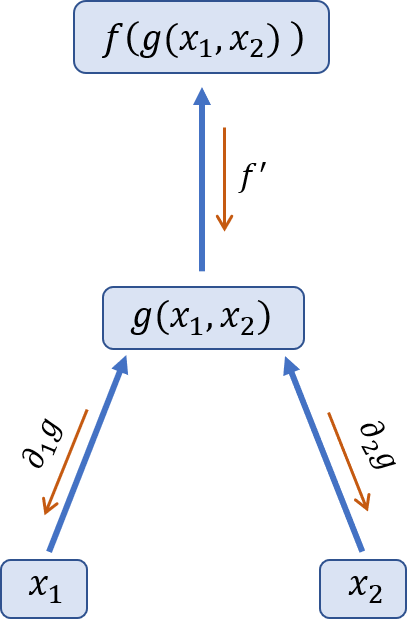
\includegraphics[height=1.3\textwidth]{Figures/automatic-differentiation}
	\end{minipage}\hfill
	\begin{minipage}{0.3\linewidth}
		\centering
		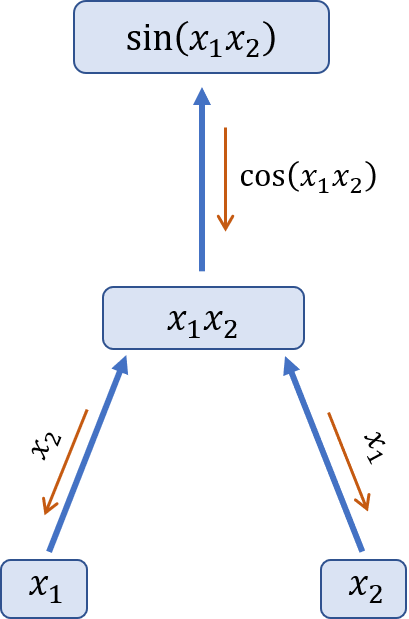
\includegraphics[height=1.3\textwidth]{automatic-differentiation2}
	\end{minipage}\hfill
	\begin{minipage}{0.3\linewidth}
		\centering
		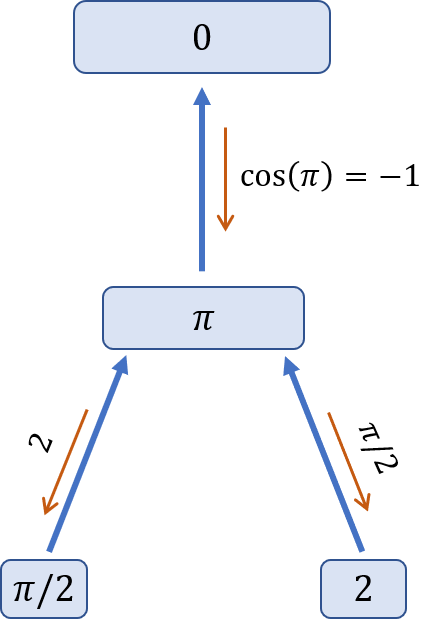
\includegraphics[height=1.3\textwidth]{automatic-differentiation3}
	\end{minipage}
	\caption{
		Examples of \ac{AD} in backpropagation mode.
		\textbf{(a)}
		Schematic representation of \ac{AD} of a function with one output and two inputs.
		Starting from numerical values for $x_1$ and $x_2$, one computes $g(x_1, x_2)$ and then $f(g(x_1, x_2))$.
		To get $\grad f(g(x_1, x_2))$, one then computes $f'(g(x_1, x_2))\partial_i g(x_1, x_2)$.
		Note that all components of this expression are known: $f'$ and $\partial_i g$ are known by assumption, and the value of $g(x_1, x_2)$ has been computed and cached in the forward propagation phase.
		\textbf{(b)} Example of application of \ac{AD} to compute the gradient of $\cos(x_1 x_2)$.
		\textbf{(c)} Using the same example function as (b), we give an example of the actual number computed at all stages when the inputs are $(x_1, x_2) = (\pi / 2, 2)$.
	}
	\label{fig:automatic-differentiation}
\end{figure}

\subsection{Implementation details}
\label{subsec:implementation_details}

% Following the surge of interest in machine learning, and in particular deep learning, in the recent years
We used python as language of choice for the implementation of the supervised learning.
Being Python language of widespread use in the machine learning community, many libraries and frameworks are available to build computational graphs over which \ac{AD} can be used.
In particular, we used \textsc{Theano}~\cite{team2016theano}, together with the \textsc{QuTiP} library for the simulation of the dynamics of quantum systems~\cite{johansson2012qutip,johansson2013qutip}.
% The code used, together with a number of usage examples, is available on GitHub (\href{https://github.com/lucainnocenti/quantum-gate-learning}{Link}).

Our implementation allows the training of an arbitrary target gate, parametrised via a time-independent Hamiltonian $\mathcal H(\bs\lambda)$.
The parametrisation is completely arbitrary (provided the dependence on the parameters is linear), so that the Hamiltonian can be chosen as $\mathcal H(\bs\lambda)=\sum_i \lambda_i A_i$ for any set of matrices $A_i$ and number of parameters $\lambda_i$.
This is made possible by the flexibility of \ac{AD}, which allows to automatically build an efficiently differentiable computational graph, without needing to hardcode the structure of the Hamiltonian.

The goal of the algorithm is, given a target gate $\mathcal G$ and a parametrisation for the Hamiltonian $\mathcal H(\bs\lambda)$, find the $\bs\lambda_0$ such that $\exp(i\mathcal H(\bs\lambda_0))=\mathcal G$.
We use for the purpose mini-batch \ac{SGD} with momentum.
The \emph{mini-batch} version of \ac{SGD} involves computing the gradient, at every iteration, averaging over the gradients computed for a number of states.
Making such \emph{batches} of states larger or smaller allows to enhance or decrease the variance of the gradients with respect to the input state.
The use of \emph{momentum}~\cite{ruder2016overview,goh2017momentum} involves using a modified version of~\cref{eq:updating_rule}.
The updating rule is instead given by
\begin{equation}
\begin{aligned}
	\bs v &\to \gamma \bs v + \eta \grad_{\bs\lambda} \calF(\psi, \bs\lambda), \\
	\bs\lambda &\to \bs\lambda + \bs v,
\end{aligned}
\label{eq:updating_rule_momentum}
\end{equation}
where here $\eta$ is the \emph{learning rate} and $\gamma$ the \emph{momentum}.
The use of the auxiliary parameter $\bs v$ during the training discourages sudden changes of direction, and can make the training significantly more efficient~\cite{goh2017momentum}.

While the cost function $\calF$ is always real, some of the intermediate calculations needed to compute it involve complex numbers.
While this poses no fundamental problems, many of the \ac{ML} libraries do not support \ac{AD} over functions with complex inputs or outputs.
We worked around this problem using a similar trick to the one reported in~\cite{leung2017speedup}.
In particular, to use the existing framework, we mapped the problem into one involving only real numbers.
To do this, we map complex matrices into real ones via the bijection
$A\mapsto\mathfrak{Re}(A)\equiv I \otimes A_{R} - i \sigma_y\otimes A_{I}$,
where $A_R$ and $A_I$ are the real and imaginary parts of $A$, respectively.
At the same time, state vectors are to be mapped to
$\Psi\mapsto\mathfrak{Re}(\Psi)\equiv(\Psi_R, \Psi_I)^T$.
It is easy to verify that with this mapping
$A\Psi\mapsto\mathfrak{Re}(A\Psi)=\mathfrak{Re}(A)\mathfrak{Re}(\Psi)$,
so that all calculations can be equivalently be carried out with the real versions of matrices and vectors.

More specifically, the employed algorithm involves the following steps:
\begin{enumerate}
	\item Choose an initial set of parameters $\bs\lambda$ (randomly, or specific values if one has an idea of where a solution might be).
	A number of other hyperparameters have to be decided at this step, depending on the exact \ac{SGD} method used. In particular, for mini-batch \ac{SGD} with momentum and decreasing learning rate, one has to decide the momentum $\gamma$, the initial value of $\eta$, the rate at which $\eta$ decreases during the training, and the size $N_b$ of the batches of states used for every gradient descent step.
	\item Repeat the following loop $N_e$ times, or until a satisfactory result is obtained.
	Each such iteration is conventionally named an \emph{epoch}.
	Another hyperparameter to be chosen beforehand is the number of training states $N_{tr}$ to be used in each epoch.
	Once this is fixed, every epoch will involve a number $N_{tr}/N_e$ of gradient descent steps, each one using $N_e$ states for a single gradient calculation.
	$N_e$ random training states are sampled, to be used during the epoch.
	\begin{enumerate}
		\item Pick $N_b$ of the $N_e$ training states.
		\item Forward-propagate each state of the sample, and then backpropagate the gradients, thus computing the average gradient over the mini-batch $\grad_{\bs\lambda} \calF(\bs\lambda)$.
		\item Update the coupling strengths $\lambda$ as per~\cref{eq:updating_rule_momentum}.
		\item Return to point (a).
	\end{enumerate}
\end{enumerate}

\subsection{Results}
\label{subsec:numerical_results}

A sample of training results for Toffoli, Fredkin, and "double Fredkin" gates are given in Fig. 1 (a), (b), and (c) in the main text.
In~\cref{fig:toffoli_diagonal_parhistories,fig:fredkin_diagonal_parhistories,fig:doublefredkin_diagonal_parhistories} are shown the training histories of the parameters for eight different solutions for Toffoli, Fredkin and \emph{double Fredkin}, respectively.
These illustrate how quickly the networks converge for different initial values of the parameters.
In all the shown cases the target gates are obtained with unit fidelity up to numerical precision (that is, all fidelities are between $1-10^{-16}$ and $1$).
Different sets of optimisation hyperparameters are found to give acceptable solutions.
For the trainings shown in this paper we used a dynamically updated learning rate given, for the $k^{\text{th}}$ epoch, by $\eta=1/(1 + k \alpha)$ with the \emph{decay rate} $\alpha=0.005$.
The other hyperparameters were chosen as
$\gamma=0.5$, 
$N_b = 2$, $N_{tr} = 200$.
Different initial values for the parameters were tested, but in most cases we started the training with either vanishing or random (following a normal distribution) parameters.
For the training of the four-qubit gate we found the network to converge sooner to a solution when the parameters were initialised to a positive value (often with all parameters initialised to $4$).

In~\cref{fig:toffoli_fidVSpars,fig:fredkin_fidVSpars,fig:doublefredkin_fidVSpars} we report the behaviour of the fidelity upon changes of the learnt Hamiltonian parameters, for Toffoli, Fredkin and \emph{double Fredkin} gates, respectively.
As shown in these plots, the stability of the implemented gates with respect to variations of time and interactions values greatly varies between different solutions, as well as between different parameters in the same solutions.

To assess the feasibility of nontrivial gates in more restrictive experimental scenarios, we performed a systematic analysis of the reachability of Fredkin and Toffoli gates when allowing only for single-qubit and $X_i X_j+Y_i Y_j$ two-qubit interactions, and in the less restrictive setting of allowing for all $X_i X_j$ and $Y_i Y_j$ interactions.
The results are shown in~\cref{fig:fredkin_XY,fig:fredkin_XX,fig:toffoli_XX,fig:toffoli_XY}.
For the Fredkin gate, in the more restrictive $XX$ interactions setting, the biggest fidelity obtained was $\calF\simeq 0.94$, while when allowing for all $XX$ and $YY$ interactions the maximum fidelity obtained was $\calF\simeq0.999$.
For the Toffoli gate, the maximum fidelity obtained in the $XX$ scenario was $\calF\simeq0.94$ as well, while when allowing for all $XX$ and $YY$ interactions the best training results corresponded to $\calF\simeq 0.98$.
To have more consistent results, in all the training instances shown here all the hyperparameters, except for the interaction parameters' initial values, were chosen to have the same value.
In particular, each training instance was run for $200$ epochs, each one using $200$ random quantum states as inputs, divided in batches of $2$ elements.
This choice of hyperparameters is mostly empirical, and it is possible for different values to provide better results.

The above provides further evidence for the flexibility of the supervised learning approach, which can produce solutions with good fidelities even in more restrictive scenarios, closer to the capabilities of state of the art experimental architectures.
Furthermore, the values of the interaction strengths for many of the presented solutions are found to be compatible with the capabilities of state of the art circuit-QED architectures with gate times of the order of tens of nanoseconds~\cite{potocnik2018studying}.

Additional solutions and data, as well as the code used to produce them, is available in the GitHub repository
\href{https://github.com/lucainnocenti/quantum-gate-learning-1803.07119}{lucainnocenti/quantum-gate-learning-1803.07119}.
This repository contains all the code used to reproduce the solutions presented in this paper, as well as to train arbitrary gates on arbitrary numbers of qubits.
Even more generally, arbitrary (linearly) parametrised matrices can be used as training model, allowing a high degree of flexibility.

\begin{figure}[htbp]
	\centering
	\begin{tikzpicture}
		\node[anchor=south west] (A) at (0, 0)%
			{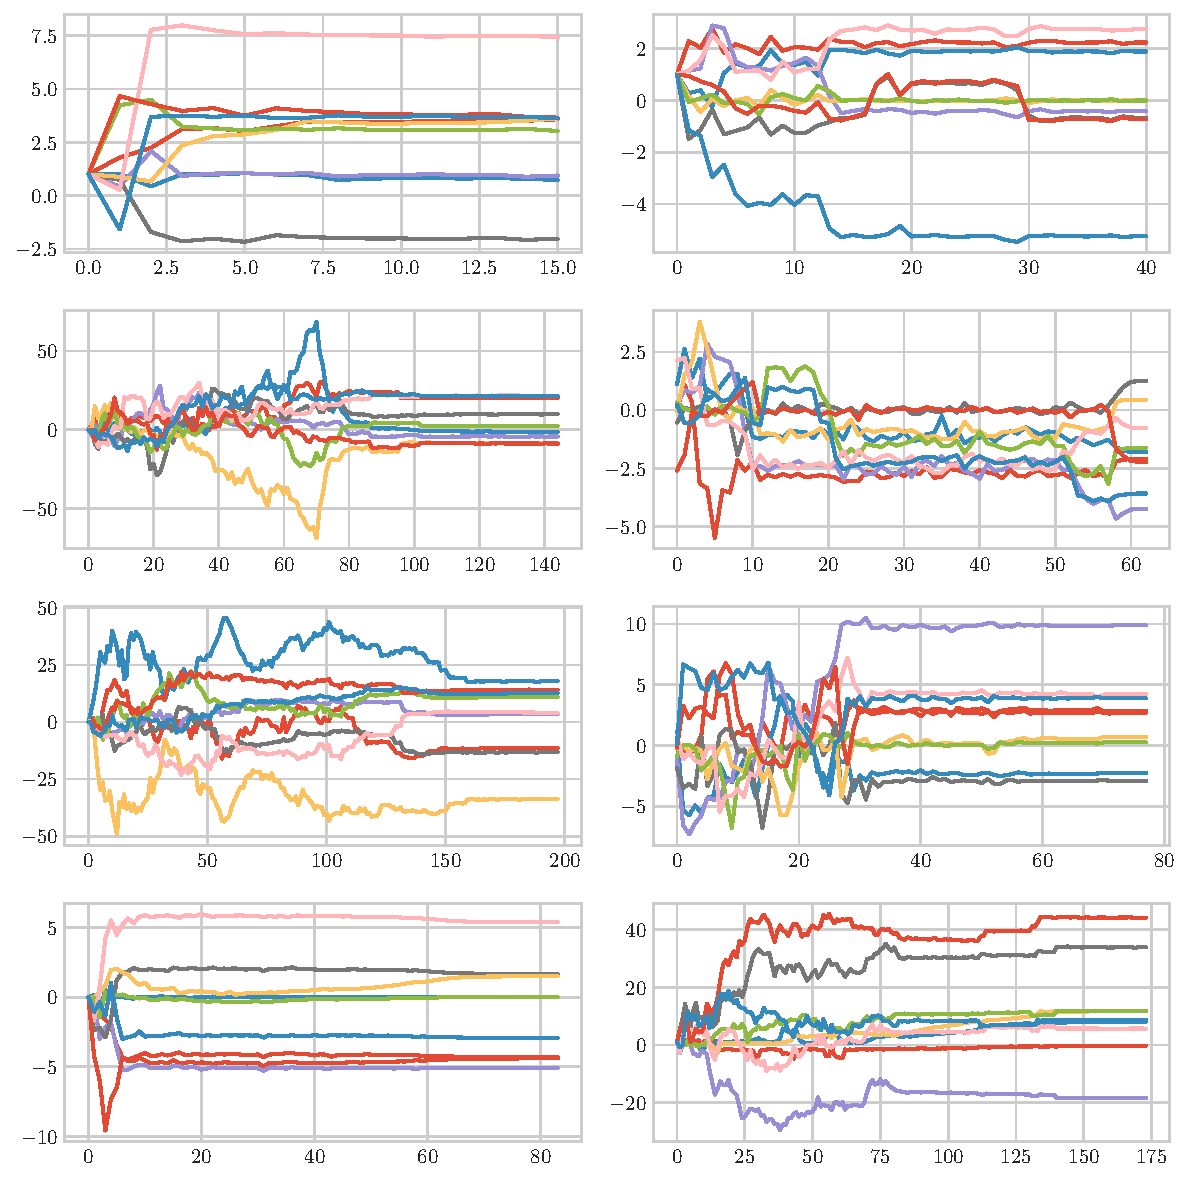
\includegraphics[width=.8\linewidth]{toffoli_diagonal_parhistories}};
		\node[above] at (4., -.2) {$t_e$};
		\node[above] at (11.5, -.2) {$t_e$};
	\end{tikzpicture}%
	% 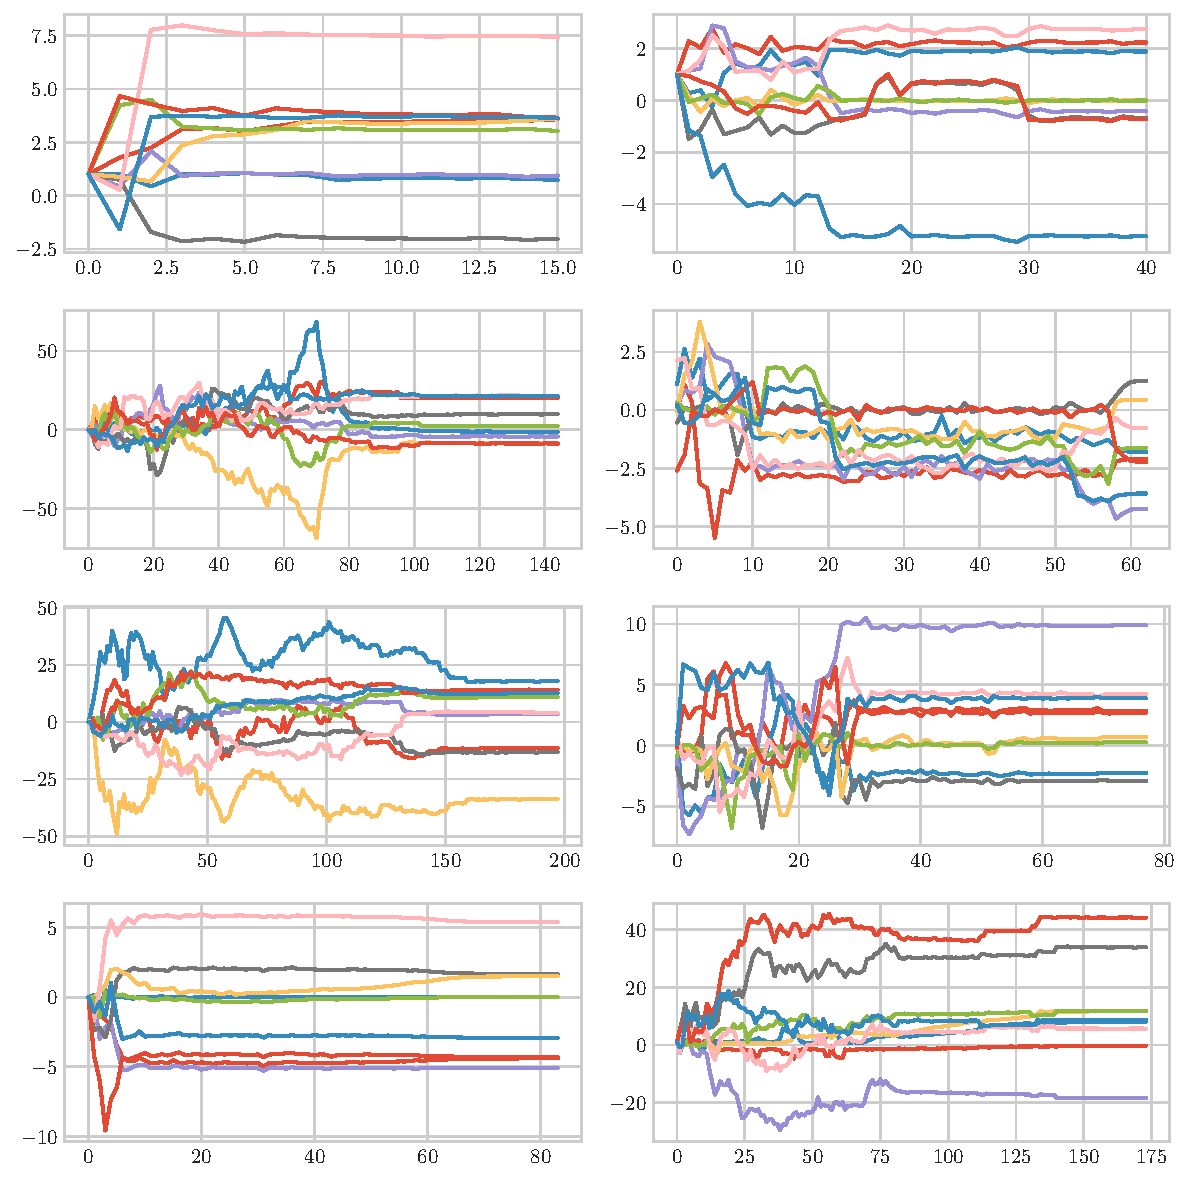
\includegraphics[width=.8\linewidth]{toffoli_diagonal_parhistories}
	\caption{
		Training histories for the \textbf{Toffoli} gate with only diagonal interactions.
		In each plot are reported the values of the $9$ network parameters during the training process, for each training epoch $t_e$.
		Each training process was left running until convergence to unit fidelity, therefore, the number of epochs in the horizontal axes differs for different trainings instances.
		The histories shown here correspond to training instances in which the parameters were initialised at various values, as seen from the leftmost values in each plot.
	}
	\label{fig:toffoli_diagonal_parhistories}
\end{figure}
 
\begin{figure}[htbp]
	\centering
		\begin{tikzpicture}
		\node[anchor=south west] (A) at (0, 0)%
			{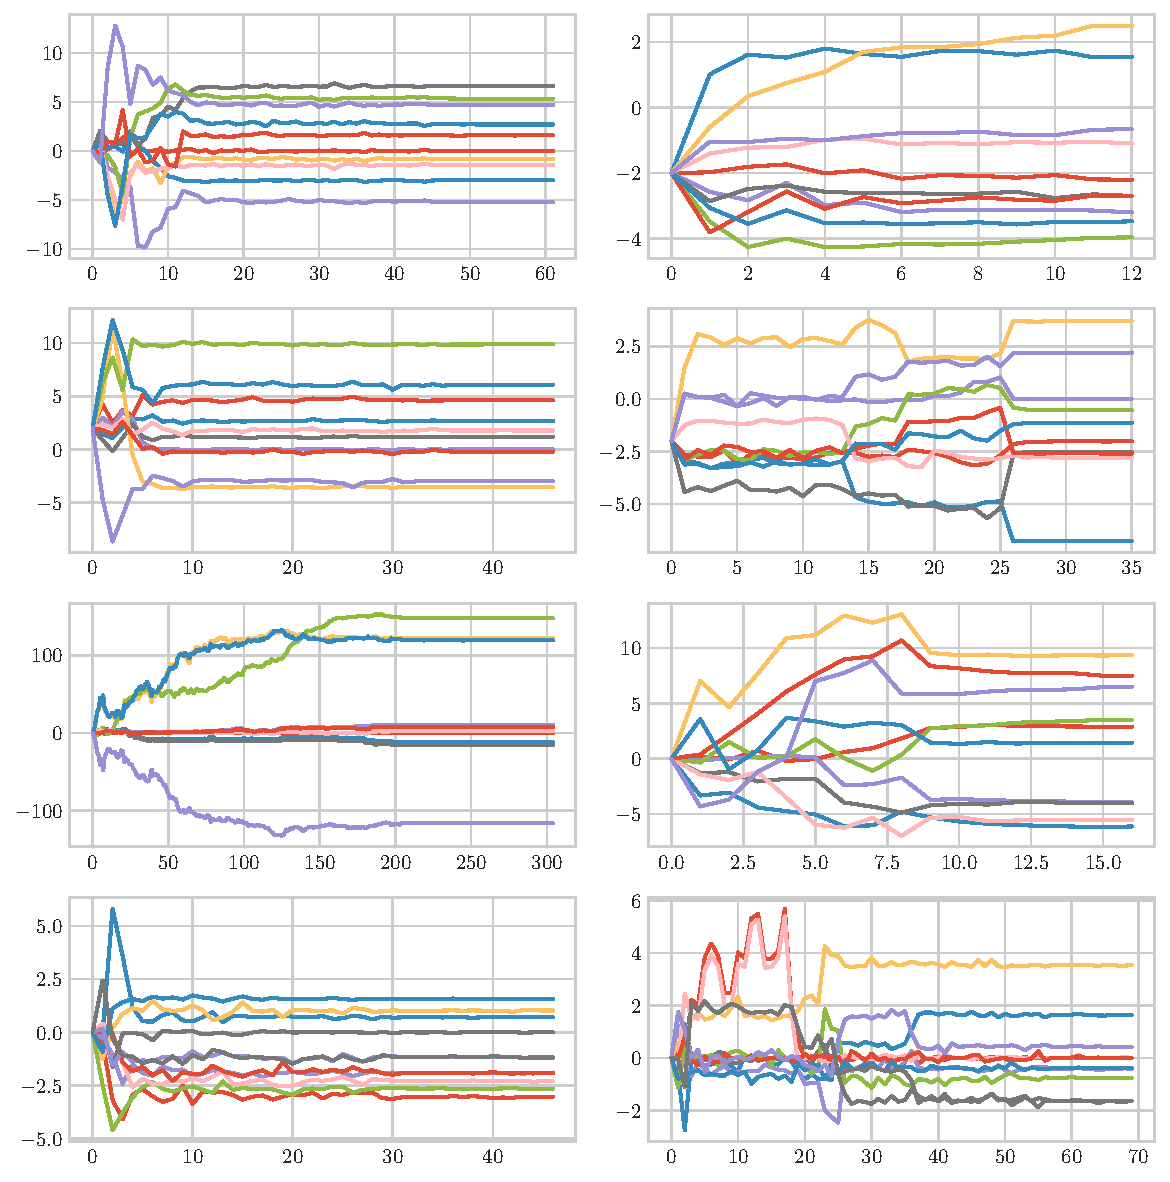
\includegraphics[width=.8\linewidth]{fredkin_diagonal_parhistories}};
		\node[above] at (4., -.2) {$t_e$};
		\node[above] at (11.5, -.2) {$t_e$};
	\end{tikzpicture}%
	% 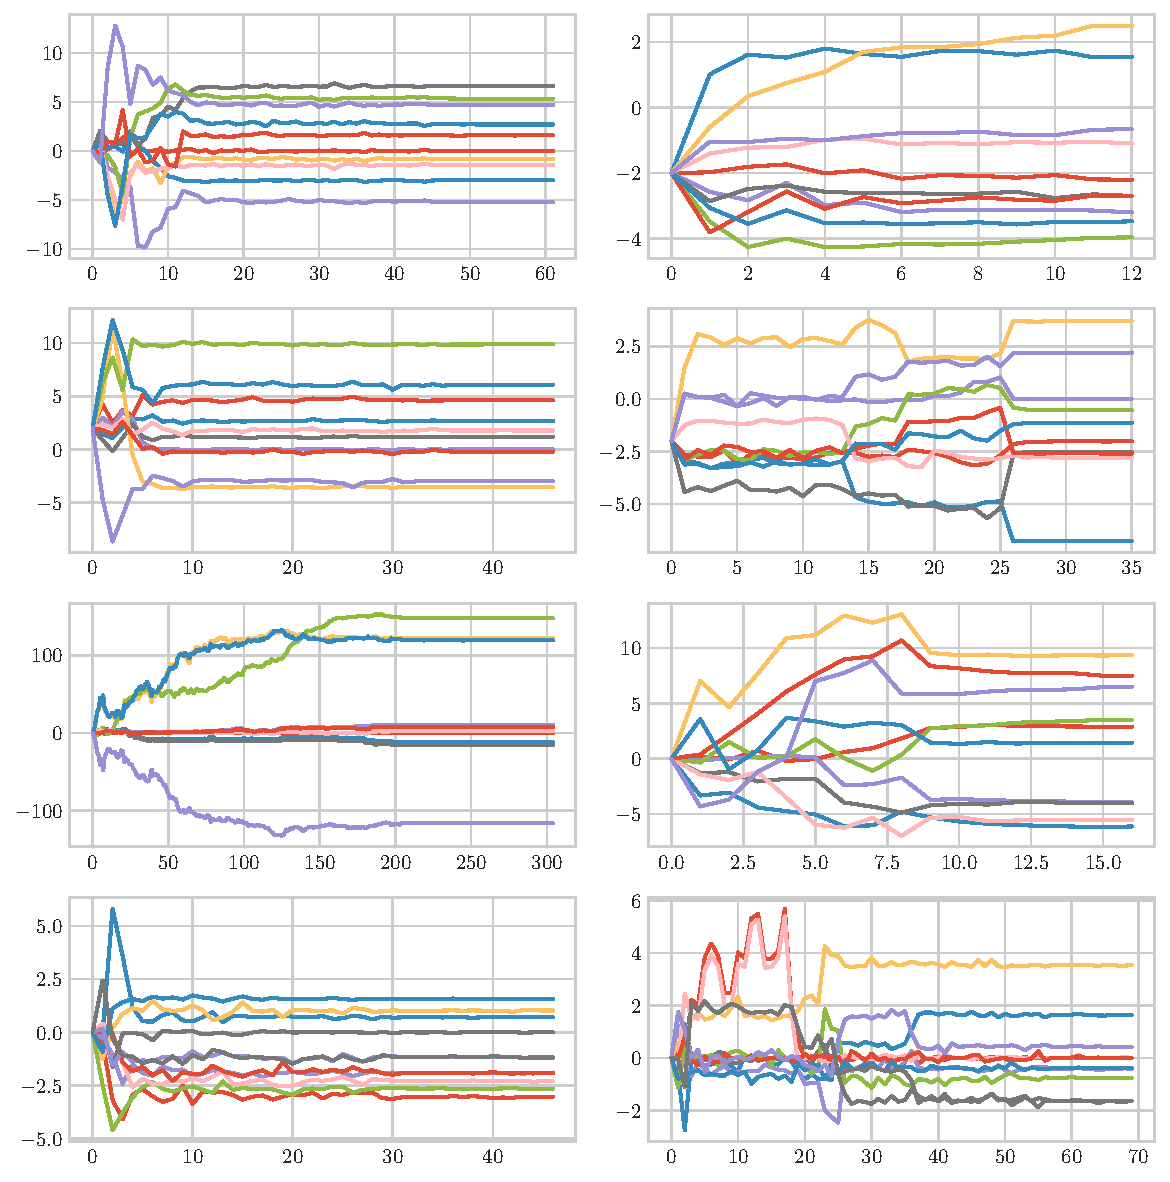
\includegraphics[width=.8\linewidth]{fredkin_diagonal_parhistories}
	\caption{
		Training histories for the \textbf{Fredkin} gate with only diagonal interactions.
		In each plot are reported the values of the $9$ network parameters during the training process, for each training epoch $t_e$.
		Each training process was left running until convergence to unit fidelity, therefore, the number of epochs in the horizontal axes differs for different trainings instances.
		The histories shown here correspond to training instances in which the parameters were initialised at various values, as seen from the leftmost values in each plot.
	}
	\label{fig:fredkin_diagonal_parhistories}
\end{figure}

\begin{figure}[htbp]
	\centering
	\begin{tikzpicture}
		\node[anchor=south west] (A) at (0, 0)%
			{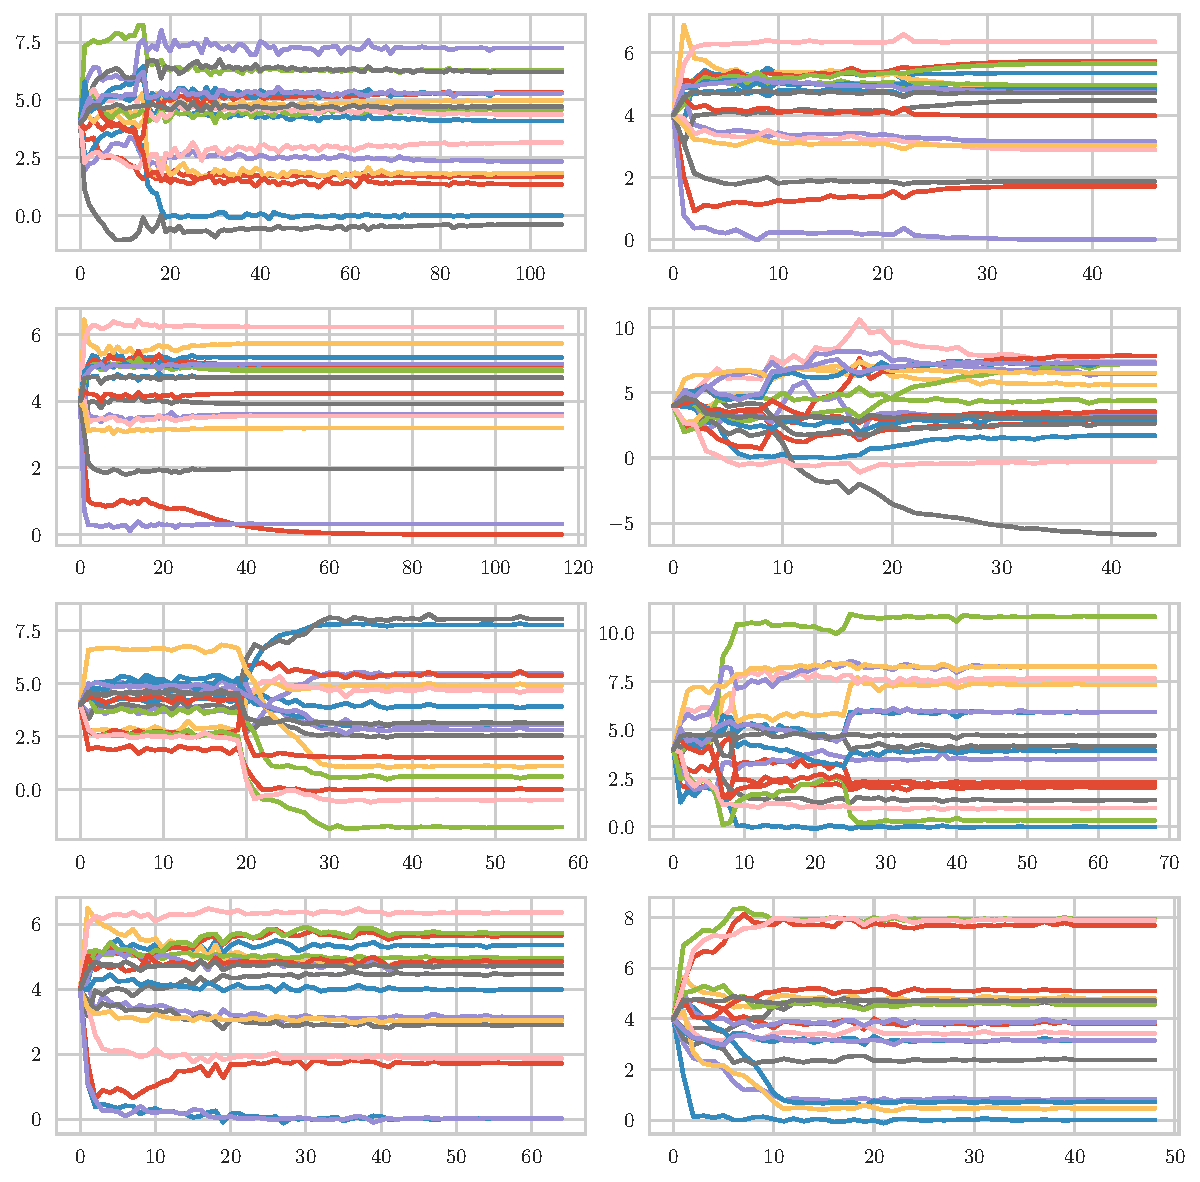
\includegraphics[width=.8\linewidth]{doublefredkin_diagonal_initvalues4_parhistories}};
		\node[above] at (4., -.2) {$t_e$};
		\node[above] at (11.5, -.2) {$t_e$};
	\end{tikzpicture}%
	% 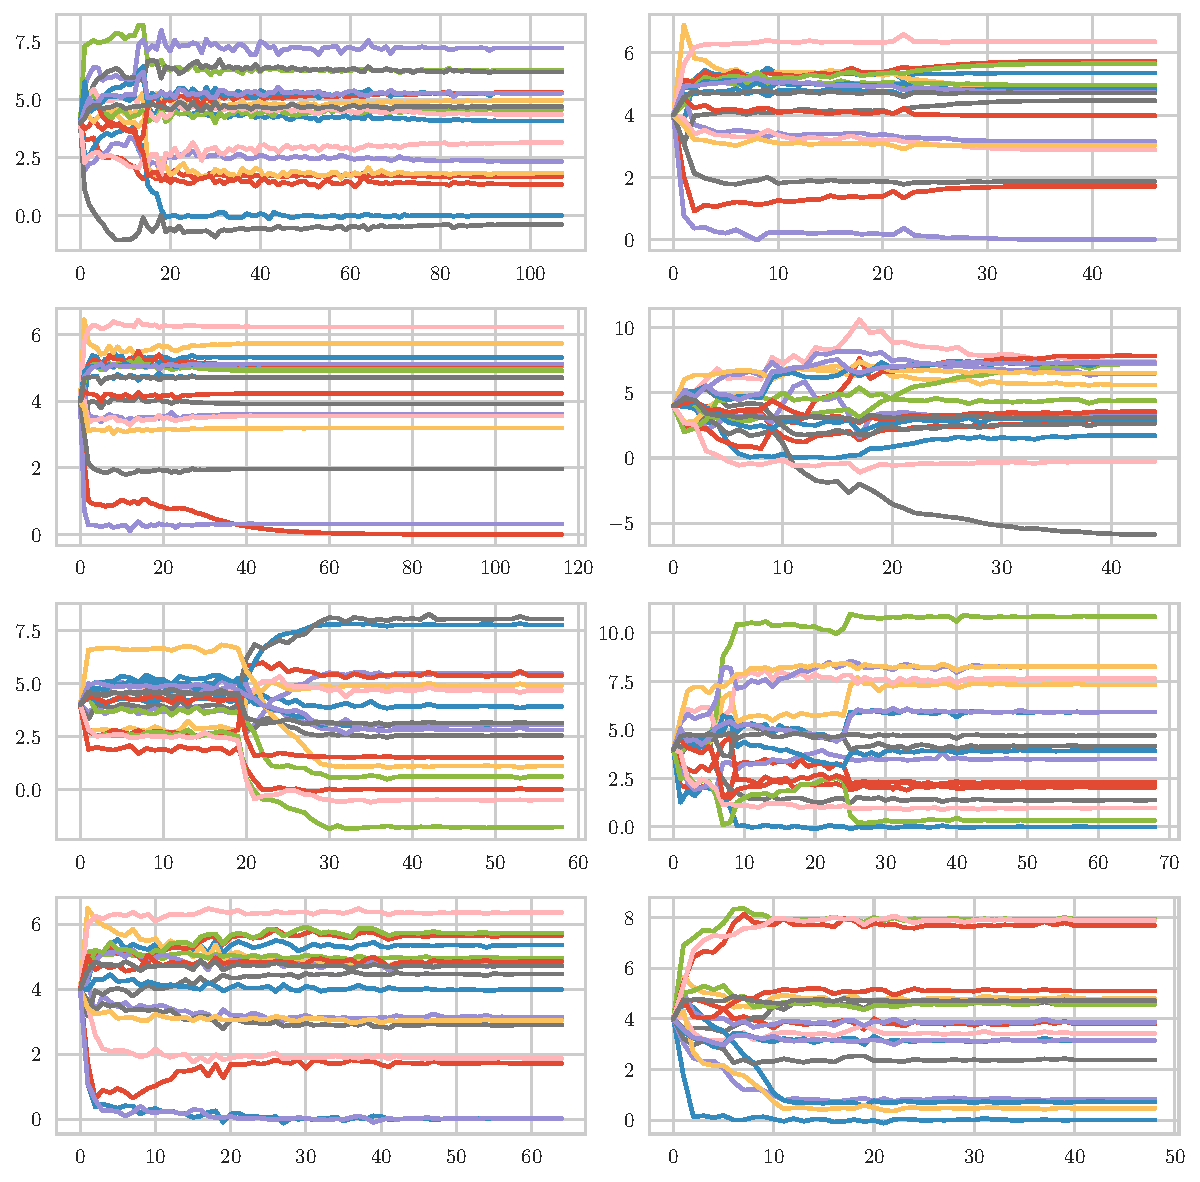
\includegraphics[width=.8\linewidth]{doublefredkin_diagonal_initvalues4_parhistories}
	\caption{
		Training histories for the \textbf{double-Fredkin} gate with only diagonal interactions.
		In each plot are reported the values of the $18$ network parameters during the training process, for each training epoch $t_e$.
		Each training process was left running until convergence to unit fidelity, therefore, the number of epochs in the horizontal axes differs for different trainings instances.
		All the histories shown here correspond to training instances in which the parameters were initialised to $4$.
	}
	\label{fig:doublefredkin_diagonal_parhistories}
\end{figure}

\newcommand{\graphicswithlabel}[3]{%
	\begin{tikzpicture}
		\node[anchor=north west] (A) at (0, 0)%
			{\includegraphics[width=.48\linewidth]{#2}};
		\node[above] at (1.4, -.85) {\small\textbf{(#1)}};
		\node[above] at (4.6, -4.65) {#3};
		\node[above] at (1., -.2) {$\calF_\bslambda(\psi)$};
	\end{tikzpicture}%
}
\begin{figure}[htbp]
	\centering
	\graphicswithlabel{a}{toffoli_fidVStime}{$\alpha$}%\vspace{-6pt}
	\graphicswithlabel{b}{toffoli_fidVStime_wide}{$\alpha$}
	\graphicswithlabel{c}{toffoli_fidVSpar0}{$\lambda_1$}\vspace{-6pt}
	\graphicswithlabel{d}{toffoli_fidVSpar1}{$\lambda_2$}
 	\caption{
 		Fidelity $\calF_\bslambda(\psi)$ vs variations of $\bslambda$, for different test states, for the \textbf{Toffoli} gate. The five test states $\psi$ are sampled randomly.
 		\textbf{(a)} Global relative variations of $\bslambda$, that is, plotting the fidelity against $\alpha\bslambda$ for $0.9 \le\alpha\le 1.1$.
 		Note that this is equivalent to studying how the fidelity changes with respect to uncertainties in the evolution time, that is, how much does $\exp(i\calH t')$ differ from $\exp(i\calH t)$.
 		\textbf{(b)} Same as \emph{(a)} but with $0\le\alpha\le 1.2$.
 		\textbf{(c)} Plot of $\calF_\bslambda(\psi)$ against \emph{absolute} variations of a single element of $\bslambda$, in this case the first one, i.e. we take $\lambda_1\in[-10,10]$.
 		\textbf{(d)} Like \emph{(c)} but for $\lambda_2$.
 	}
 %\label{fig:toffoli_fidVSpars}
\end{figure}

\renewcommand{\graphicswithlabel}[3]{%
	\begin{tikzpicture}
		\node[anchor=north west] (A) at (0, 0)%
			{\includegraphics[width=.48\linewidth]{#2}};
		\node[above] at (1.4, -.85) {\small\textbf{(#1)}};
		\node[above] at (4.6, -4.65) {#3};
		\node[above] at (1., -.2) {$\calF_\bslambda(\psi)$};
	\end{tikzpicture}%
}
\begin{figure}[htbp]
	\centering
	\graphicswithlabel{a}{fredkin_fidVStime}{$\alpha$}\vspace{-6pt}
	\graphicswithlabel{b}{fredkin_fidVStime_wide}{$\alpha$}
	\graphicswithlabel{c}{fredkin_fidVSpar0}{$\lambda_1$}\vspace{-6pt}
	\graphicswithlabel{d}{fredkin_fidVSpar3}{$\lambda_2$}
	\caption{
		Fidelity $\calF_\bslambda(\psi)$ vs variations of $\bslambda$, for different test states, for the \textbf{Fredkin} gate. The five test states $\psi$ are sampled randomly.
		\textbf{(a)} Global relative variations of $\bslambda$, that is, plotting the fidelity against $\alpha\bslambda$ for $0.9 \le\alpha\le 1.1$.
		Note that this is equivalent to studying how the fidelity changes with respect to uncertainties in the evolution time, that is, how much does $\exp(i\calH t')$ differ from $\exp(i\calH t)$.
		\textbf{(b)} Same as \emph{(a)} but with $0\le\alpha\le 1.2$.
		\textbf{(c)} Plot of $\calF_\bslambda(\psi)$ against \emph{absolute} variations of a single element of $\bslambda$, in this case the first one, i.e. we take $\lambda_1\in[-10,10]$.
		\textbf{(d)} Like \emph{(c)} but for $\lambda_2$.
	}
	\label{fig:fredkin_fidVSpars}
\end{figure}

\renewcommand{\graphicswithlabel}[3]{%
	\begin{tikzpicture}
		\node[anchor=north west] (A) at (0, 0)%
			{\includegraphics[width=.48\linewidth]{#2}};
		\node[above] at (1.4, -.85) {\small\textbf{(#1)}};
		\node[above] at (4.6, -4.65) {#3};
		\node[above] at (1., -.2) {$\calF_\bslambda(\psi)$};
	\end{tikzpicture}%
}
\begin{figure}[htbp]
	\centering
	\graphicswithlabel{a}{doublefredkin_fidVStime}{$\alpha$}\vspace{-6pt}
	\graphicswithlabel{b}{doublefredkin_fidVStime_wide}{$\alpha$}
	\graphicswithlabel{c}{doublefredkin_fidVSpar0}{$\lambda_1$}\vspace{-6pt}
	\graphicswithlabel{d}{doublefredkin_fidVSpar1}{$\lambda_2$}
	\caption{
		Fidelity $\calF_\bslambda(\psi)$ vs variations of $\bslambda$, for different test states, for the \textbf{double Fredkin} gate. The five test states $\psi$ are sampled randomly.
		\textbf{(a)} Global relative variations of $\bslambda$, that is, plotting the fidelity against $\alpha\bslambda$ for $0.9 \le\alpha\le 1.1$.
		Note that this is equivalent to studying how the fidelity changes with respect to uncertainties in the evolution time, that is, how much does $\exp(i\calH t')$ differ from $\exp(i\calH t)$.
		\textbf{(b)} Same as \emph{(a)} but with $0\le\alpha\le 1.2$.
		\textbf{(c)} Plot of $\calF_\bslambda(\psi)$ against \emph{absolute} variations of a single element of $\bslambda$, in this case the first one, i.e. we take $\lambda_1\in[-10,10]$.
		\textbf{(d)} Like \emph{(c)} but for $\lambda_2$.
	}
	\label{fig:doublefredkin_fidVSpars}
\end{figure}


\newcommand{\traininggraphicswithlabel}[1]{%
	\begin{tikzpicture}
		\node[anchor=north west] (A) at (0, 0)%
			{\includegraphics[width=.85\linewidth]{#1}};
		\node[above] at (0, -.8) {$\barF$};
	\end{tikzpicture}%
}

\begin{figure}[htbp]
	\centering
	% 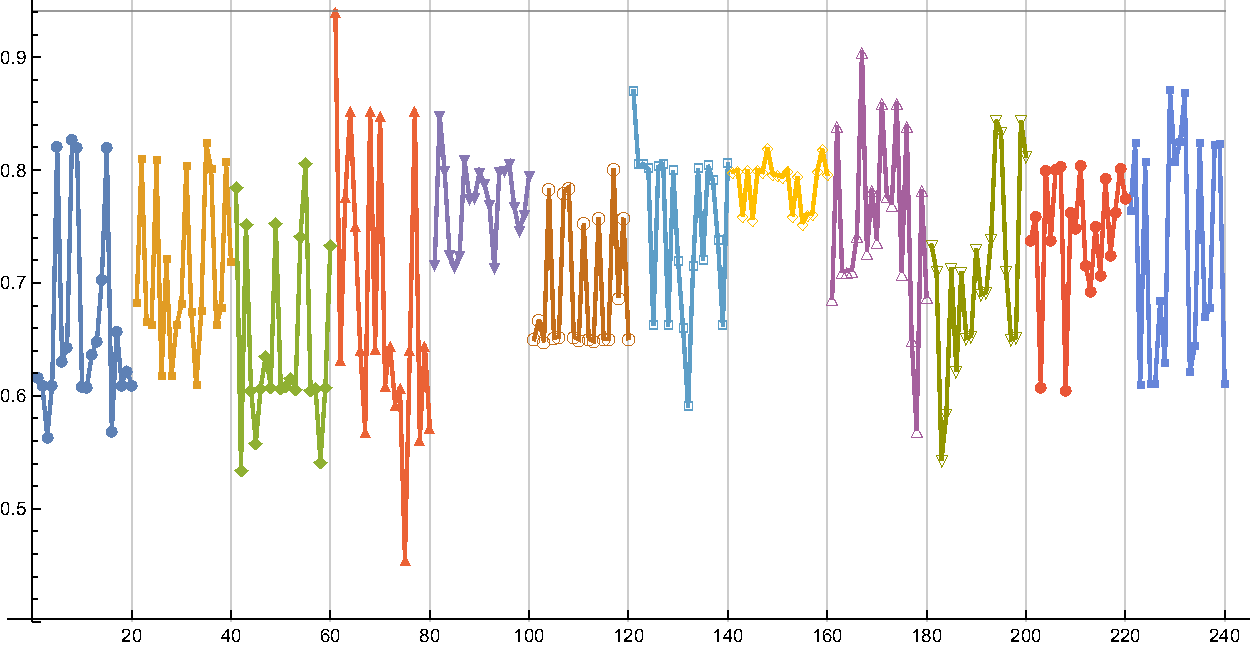
\includegraphics[width=.85\linewidth]{fredkin_noancillae_XXall.pdf}
	\traininggraphicswithlabel{fredkin_noancillae_XXall.pdf}
	\caption{
		Training results for the Fredkin gate with a generator containing one-qubit interactions and two-qubit interactions of the form $J_{ij}(X_i X_j + Y_i Y_j)$.
		Every point shows the final fidelity obtained at the end of a training procedure.
		The hyperparameters, as well as the total number of training iterations, are kept the same in all the training instances shown here.
		The initial parameters' values are the same within each horizontal sector, but changed between different sectors.
		The initial parameters' values within each sector have been chosen as all equal to $c$ (that is, $\lambda_i=c$ for all $i$). The values of $c$ are $0, 1,\ldots, 10$, with $c=0$ in the leftmost sector and $c=10$ in the last to rightmost one.
		The rightmost sector contains the results of training attempts with the initial values chosen at random (that is, with $\lambda_i$ sampled according to the uniform normal distribution, independently for each $i$).
		The greatest reached fidelity, obtained with initial parameters' values $\lambda_i=3$, is $\calF\simeq0.94$.
	}
\label{fig:fredkin_XX}
\end{figure}

\begin{figure}[htbp]
	\centering
	\traininggraphicswithlabel{fredkin_noancillae_XYall.pdf}
	\caption{
		Training results for the Fredkin gate with a generator containing all one-qubit interactions and two-qubit interactions of the form $J^{(1)}_{ij}X_i X_j + J^{(2)}_{ij}Y_i Y_j$.
		The initial conditions are chosen as in~\cref{fig:fredkin_XX}.
		The maximum fidelities obtained are $\calF\simeq0.999$, obtained in multiple instances $c=3$ and $c=4$ sectors.
	}
\label{fig:fredkin_XY}
\end{figure}

\begin{figure}[htbp]
	\centering
	\traininggraphicswithlabel{toffoli_noancillae_XXall.pdf}
	\caption{
		Training results for the Toffoli gate with a generator containing all one-qubit interactions and two-qubit interactions of the form $J_{ij}(X_i X_j + Y_i Y_j)$.
		The initial conditions are chosen as in~\cref{fig:fredkin_XX}.
		The maximum fidelities obtained are $\calF\simeq0.94$, obtained in the $c=3$ sector.
	}
	\label{fig:toffoli_XX}
\end{figure}

\begin{figure}[htbp]
	\centering
	\traininggraphicswithlabel{toffoli_noancillae_XYall.pdf}
	\caption{
		Training results for the Toffoli gate with a generator containing all one-qubit interactions and two-qubit interactions of the form $J^{(1)}_{ij}X_i X_j + J^{(2)}_{ij}Y_i Y_j$.
		The initial conditions are chosen as in~\cref{fig:fredkin_XX}.
		The maximum fidelities obtained are $\calF\simeq0.98$, obtained in the $c=4$ and $c=5$ sectors.
	}
	\label{fig:toffoli_XY}
\end{figure}

\subsection{Numerical approximate results in constrained scenarios}

% \EnableTOCUpdates
